\documentclass[onecolumn, fleqn]{article}
\usepackage[letterpaper, margin=1in]{geometry}

\usepackage{epsf}
%\usepackage{times}
\usepackage{latexsym}
\usepackage{amsbsy}
\usepackage{ifthen}

%\usepackage[sort&compress,square,comma,authoryear]{natbib}
%\usepackage[round]{natbib}
\usepackage{color, soul}
\usepackage{fancyhdr}	% Package to create Headers and Footers
\usepackage{tabu, tabulary, tabularx} 	% packages for tables
\usepackage{multirow}
\usepackage{float}
\usepackage{booktabs}
\usepackage{enumerate, enumitem}
\usepackage[pdftex]{graphicx}
\usepackage[hypcap,justification=centerlast,labelfont=bf,font=small]{caption}
\usepackage{pdflscape}
\usepackage{xfrac}
\usepackage{arydshln}
%\usepackage[sc]{titlesec}
\usepackage{subcaption}
\usepackage{hyperref}
\usepackage{amsmath,amssymb,mathrsfs}
\usepackage{epstopdf}
%\usepackage[tight,footnotesize]{subfigure}
\usepackage{dcolumn}
\usepackage{bm}
\usepackage[super]{nth}
\usepackage{todonotes}
\usepackage{pdfpages}
\usepackage[numbers,sort]{natbib}
\usepackage[capitalize,nameinlink,noabbrev]{cleveref}
%\usepackage[round]{natbib}   % omit 'round' option if you prefer square brackets
%\bibliographystyle{plainnat}
\usepackage{hyperref}
\hypersetup{
  colorlinks   = true,    % Colors links instead of ugly boxes
  urlcolor     = blue,    % Color for external hyperlinks
  linkcolor    = blue,    % Color of internal links
  citecolor    = blue      % Color of citations
}





% Commands %%%%%
	\newcommand{\mb}[1]{$\mathbf{#1}$}
	\newcommand{\bs}[1]{\boldsymbol #1}
	\newcommand{\intwo}{\ensuremath{\,\mathrm{in}^2}}
	\newcommand{\ksi}{\ensuremath{\,\mathrm{ksi}}}
	\newcommand{\kip}{\ensuremath{\,\mathrm{k}}}
	\newcommand{\psf}{\ensuremath{\,\mathrm{psf}}}
	\newcommand{\kips}{\ensuremath{\,\mathrm{kips}}}
	\newcommand{\ftk}{\ensuremath{\,\mathrm{ft-k}}}
	\newcommand{\ink}{\ensuremath{\,\mathrm{in-k}}}
	\newcommand{\ft}{\ensuremath{\,\mathrm{ft}}}
	\newcommand{\m}{\ensuremath{\,\mathrm{m}}}
	\newcommand{\inch}{\ensuremath{\,\mathrm{in}}}
	\newcommand{\pdiff}[2]{\frac{\partial#1}{\partial#2}}
	\newcommand{\solution}[1]{\color{blue!40!black}{\fbox{\begin{minipage}{0.933\textwidth}
								{#1}\end{minipage}}}\color{black}}
	
	\newcommand{\atena}{ATENA}

%%%%%%%% TITLE %%%%%%%%
\DeclareFixedFont{\bigsf}{OT1}{cmr}{b}{sc}{25}%{T1}{cmr}{b}{sc}{0.5in}
%\title{\bigsf{Investigation of Stiffness Irregularity in RC Walls}}
\title{\bigsf{EVW Tool Examples}}
\date{}
%\author{Kamal A. Ahmed}






%%%%%%%%%%%%%%%%%%%%%%%%%%%%%%%%%%%%%%%%%%%%%%%%%%%%%%%%%%%%%%%%%%%%%%%%%%%%%%%%%%
%					Beginning the document										 %
%%%%%%%%%%%%%%%%%%%%%%%%%%%%%%%%%%%%%%%%%%%%%%%%%%%%%%%%%%%%%%%%%%%%%%%%%%%%%%%%%%

\begin{document}
\maketitle
\addcontentsline{toc}{section}{Front Page}

\newpage
%\tableofcontents
%\addcontentsline{toc}{section}{Contents}

\graphicspath{{figures/}{}}

Examples included in this document employ the theories that are explained in the documentation (\href{https://simcenter.designsafe-ci.org/media/filer_public/a0/68/a068ba45-6a47-46f4-83b1-fae585d8ccbe/evw_documentation.pdf}{\textit{user manual}}) provided on \href{https://simcenter.designsafe-ci.org/learning-tools/evw-application/}{EVW Application Webpage}.

\renewcommand{\thesection}{Example \arabic{section}:}
\renewcommand{\thesubsection}{Example \arabic{subsection}:}

\section{The SAC 3-story Los Angeles Building, Hazard Level 2/50 (3LA250)}
Building properties and loadings are adopted from SAC examples provieded in \textit{State of the Art Report on Systems Performance of Steel Moment Frames Subject to Earthquake Ground Shaking} (\citet{FEMA335c2000}). Building floor plans and elevations are shown in \cref{fig:floor_plan_elev}. Only the \textsl{North-South} direction is taken into consideration. Layout of the moment resisting building for the LA building is shown in \cref{fig:MRF_LASE}.
The loading used for the analysis of the frames is based on the details given in \citet{FEMA335c2000}, which result in the following floor load distribution (steel weight is assumed as 13 psf for all designs):

\begin{itemize}
\item[] Floor dead load for weight calculations: 96 psf
\item[] Floor dead load for mass calculations:  86 psf
\item[] Roof dead load excluding penthouse:  83 psf
\item[] Penthouse dead load:  116 psf
\item[] Reduced live load per floor and for roof: 20 psf
\end{itemize}

%Total weight of the 3-story building is: $(96 \times 2 + 83) \times 180 \times 120 + 116 \times 30 \times 60 = 6148.8 \kips$
%
%Total weight of the 20-story building is: $(96 \times 19 + 83) \times 120 \times 120 + 116 \times 20 \times 40 = 27553.6 \kips$

\begin{figure}[H]
	\centering 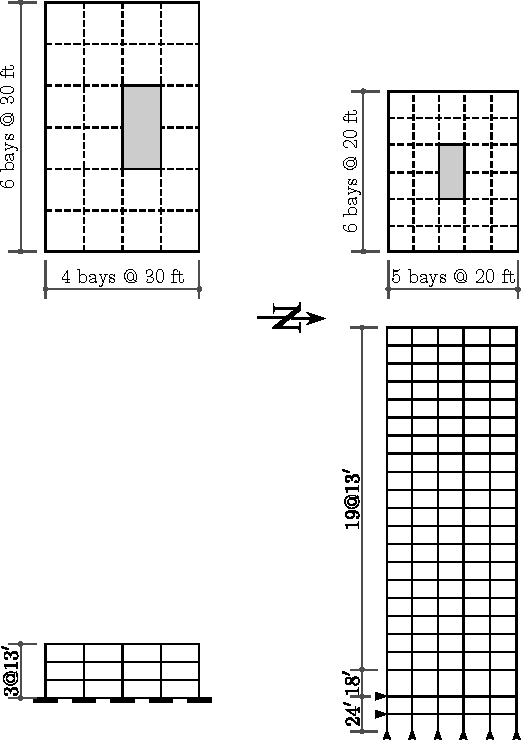
\includegraphics[width=0.45\linewidth]{SAC_floor_plans.pdf}
	\caption{Floor plans and elevations for model buildings \citep{FEMA335c2000}.}
	\label{fig:floor_plan_elev}
\end{figure}

%\begin{figure}[H]
%	\centering 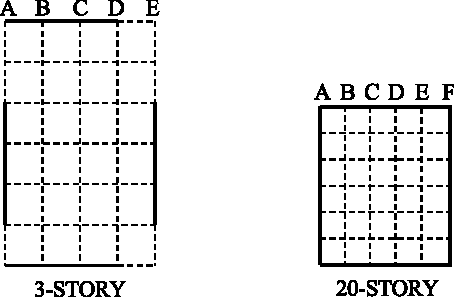
\includegraphics[width=0.55\linewidth]{SAC_moment_frame_LA.pdf}
%	\caption{Floor plans showing layout of moment-resisting frames for LA model buildings \citep{FEMA335c2000}.}
%	\label{fig:MRF_LASE}
%\end{figure}

\begin{figure}[H]
	\centering 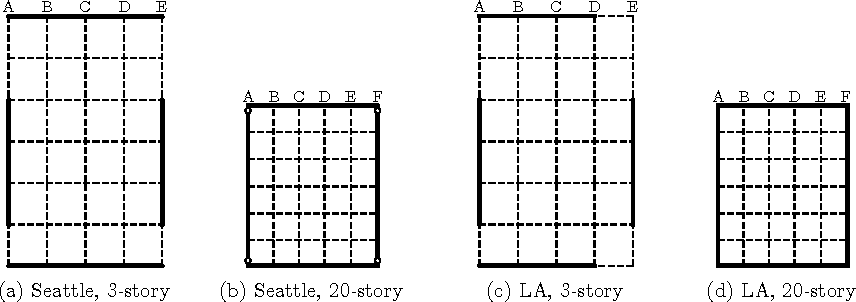
\includegraphics[width=0.8\linewidth]{SAC_moment_frame_LASE.pdf}
	\caption{Floor plans showing layout of moment-resisting frames for LA and Seattle model buildings \citep{FEMA335c2000}.}
	\label{fig:MRF_LASE}
\end{figure}


%\section*{3 Story Building, (Hazard Level 2/50)}
%Building floor plans, layout, elavation and beam and column sections can be found in Appendices A and B of the FEMA 335c.
%\\
%\textbf{Building properties} (FEMA 335c, appendices A and B)
%\begin{description}
%\item Basic wind speed at reference height in exposure C = 95 mph
%\item Type of exposure = B
%\item Building height $h = 39\ft (11.87\m)$
%\item Building width $B = 180\ft (54.79\m)$
%\item Building depth $L = 120\ft (36.53\m)$
%\item Building natural frequency $n_1 = 0.62$ Hz (\textit{for approximate natural frequencies see section 26.11.2 and C26.11 of the ASCE 7-16})
%\item Damping ratio $\zeta = 0.02$
%\item Mean along-wind force coefficient $C_\mathrm{fx} = 1.3$
%\item Mode exponent $= 1.0$
%\item Building density $\mathrm{\dfrac{mass}{volume}} = 1.03 \,\mathrm{slugs/ft^3}$
%\item Air density $= 0.0024 \,\mathrm{slugs/ft^3}$
%\end{description}

Properties of the 3-story building located in LA for the hazard level of 2/50 are tabulated in \cref{tab:prop_3LA250}. These properties are based on the location, geometry and function of the building as described in \citet{FEMA335c2000}.

\begin{table}[H]
\centering \caption{3-story building properties, Los Angeles, hazard level: 2/50 (3LA250).}
\label{tab:prop_3LA250}
\begin{tabular}{llc}
\toprule
Item		& Value		& Source		\\
\midrule
Basic wind speed at reference height in exposure C	& 95 mph						& Fig. 26.5-1 ASCE 7-16		\\
Type of exposure									& $B$							& user spec					\\
$h$ Building height									& $39\ft \,(11.87\m)$			& user spec					\\
$B$ Building width									& $180\ft \,(54.79\m)$			& user spec					\\
$L$ Building depth									& $120\ft \,(36.53\m)$			& user spec					\\
$n_1$ Building natural frequency					& $0.62$ Hz						& analysis or rational approximation$^{1)}$\\
$\zeta$ Damping ratio								& $0.02$						& rational assignment$^{2)}$		\\
$C_{fx}$ Mean along-wind force coefficient			& $1.3$							& 							\\
$\beta$ Mode exponent								& $1.0$							& user spec					\\
Building density									& $1.03 \,\mathrm{slugs/ft^3}$	& bldg function				\\
%Air density											& $0.0024 \,\mathrm{slugs/ft^3}$& bldg location				\\
\bottomrule
\multicolumn{3}{l}{\footnotesize $^{1)}$ for approximate natural frequencies see section 26.11.2 and C26.11 of the ASCE 7-16. For this example, since the building}	\\
\multicolumn{3}{l}{\footnotesize \hspace{3mm} are designed and the properties of the building elements are known, the natural frequency is accurately calculated.}	\\
\multicolumn{3}{l}{\footnotesize $^{2)}$ recommended values for damping ratio can be found in Table 11.2.1, Dynamics of Structures by
Chopra, 4th ed. \citep{ChopraAnilK2012Dos}}
\end{tabular}
\end{table}

\noindent\textbf{Procedure}\\
In order to use the \href{https://simcenter.designsafe-ci.org/learning-tools/evw-application/}{EVW app}, input forces and building properties need to be known. For Gust wind speed, gust-effect factor should be computed based on the location and function of the building according to the chapter 26 of the \citet{asce7_2016}. This is shown in \cref{tab:gust_factor_3LA250}.

\begin{table}[H]
\centering \caption{Gust-effect factor, 3LA250.}
\label{tab:gust_factor_3LA250}
\begin{tabular}{llc}
\toprule
Item		& Value		& Source		\\
\midrule
\multicolumn{3}{l}{\textbf{FLEXIBLE BUILDING} (all $n_1$)}	\\
$\bar{z}$ Effective structure height							& $23.4 \ft$					& $0.6h$ (26.11.4 ASCE 7-16)	\\
$I_{\bar{z}}$ Turbulence intensity at eff. height				& $0.318$						& eq. 26.11.7 ASCE 7-16			\\
$L_{\bar{z}}$ Turbulence length scale at eff. height			& $285.4 \ft$					& eq. 26.11.9 ASCE 7-16			\\
$V$ Basic wind speed											& $95$ mph						& Fig. 26.5-1 ASCE 7-16			\\
$\beta$ Damping ratio											& $0.02$						& rational assignment			\\
$\bar{\alpha}$ Power law exponent of mean wind speed profile	& $0.25$						& Table 26.11-1 ASCE 7-16		\\
$\bar{b}$ Gust factor 1/F at 10 m								& $0.45$						& Table 26.11-1 ASCE 7-16		\\
$\bar{V}_{\bar{z}}$ Mean wind speed at effective height			& $57.5$						& eq. 26.11-16 ASCE 7-16		\\
$N_1$ Reduced natural frequency									& $3.08$						& eq. 26.11-14 ASCE 7-16		\\
$R_n$ Resonance response factor for n							& $0.069$						& eq. 26.11-13 ASCE 7-16		\\
$\eta_h$ Vertical decay parameter								& $1.934$						& eq. 26.11-5 ASCE 7-16			\\
$\eta_B$ Cross-wind decay parameter								& $8.928$						& eq. 26.11-5 ASCE 7-16			\\
$\eta_L$ Along-wind decay parameter								& $19.926$						& eq. 26.11-5 ASCE 7-16			\\
$R_h$ Resonant factor for $h$									& $0.386$							& eq. 26.11-15a ASCE 7-16			\\
$R_B$ Resonant factor for $B$									& $0.106$							& eq. 26.11-15a ASCE 7-16			\\
$R_L$ Resonant factor for $L$									& $0.049$							& eq. 26.11-15a ASCE 7-16			\\
$R^2$ Resonant response (squared)								& $0.078$							& eq. 26.11-12 ASCE 7-16			\\
$g_R$ Resonant peak factor										& $4.074$							& eq. 26.11-11 ASCE 7-16			\\
$G_f$ Gust-effect factor										& $1.162$							& eq. 26.11-10 ASCE 7-16			\\
\bottomrule
\end{tabular}
\end{table}

Therefore, Gust wind speed in mph is:
\begin{equation*}
G_f \times C = 1.162 \times 95 = \boxed{110.4}
\end{equation*}

%In the SAC case studies, the ground motions were scaled such that, on average, their spectral values match with a least square error fit to the USGS's mapped values at 0.3, 1.0, and 2.0 seconds, and an additional predicted value at 4.0 seconds \citep{FEMA335c2000}. For the 3-story building located in Los Angeles, the scale factor is $0.79$.

For earthquake analysis and stick model, buildings can be idealized with mass concentrated at one location for each floor ($m$) and stiffness of each floor ($k$) represents the lateral stiffness of the moment resisting frames and/or walls in the direction considered. Idealized building mass and stiffness of the 3-story and 20-story buildings are shown in \cref{fig:ideal_mass_stiffness}.

\begin{figure}[H]
	\begin{subfigure}[b]{0.45\linewidth}
		\centering 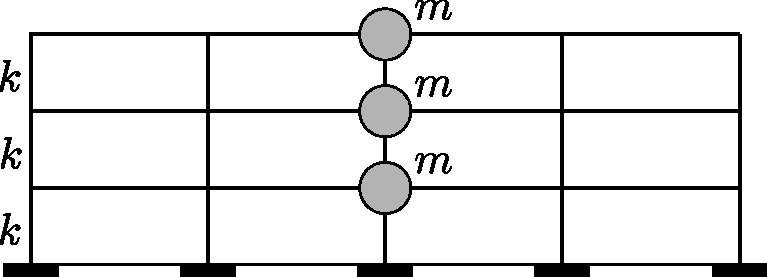
\includegraphics[scale=0.4]{3LA550_mass_model.pdf}
		\caption{3-story building}
	\end{subfigure}
	\begin{subfigure}[b]{0.45\linewidth}
		\centering 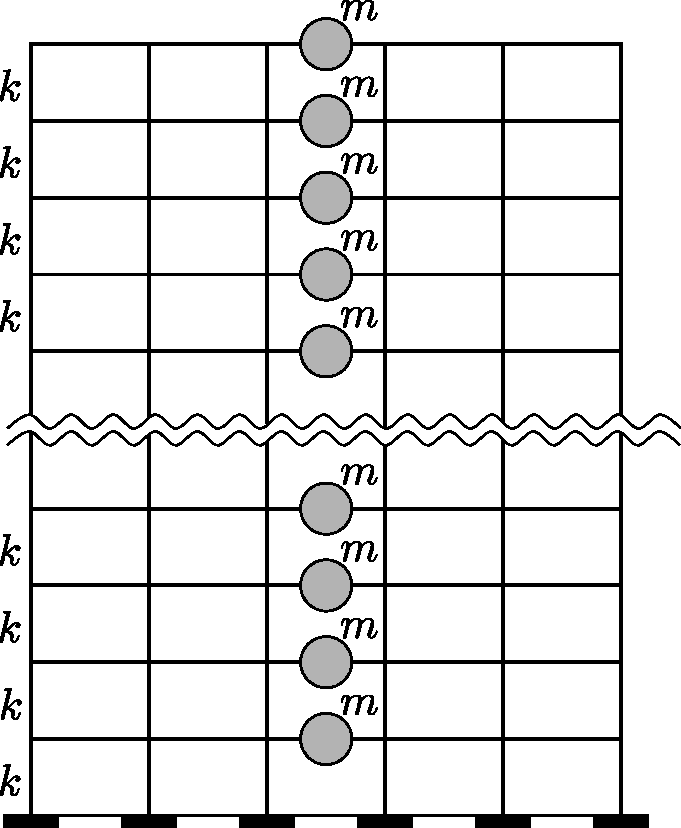
\includegraphics[scale=0.4]{20LA550_mass_model.pdf}
		\caption{20-story building}
	\end{subfigure}
\caption{Idealized building mass and stiffness}
\label{fig:ideal_mass_stiffness}
\end{figure}

%With $m$ and $n_1$ being mass in kips and natural frequency in seconds respectively, then the stiffness $K$ can be calculated as:
%\begin{equation*}
%K = \frac{4 \pi^2 m}{n_1} = \frac{4 \pi^2 (2289.6)}{1.61} = 34871.3 \kip/\mathrm{s}
%\end{equation*}

\vspace{10mm}
\noindent\textbf{Stiffness Calculation:}\\
\indent For the exact calculation of the stiffness of any structure, properties and geometry of beams, columns, walls and slabs and lateral systems need to be known. However, these information are not available prior to design. Therefore, the stiffness is usually estimated. For a single degree of freedom (SDOF) frame structure (\cref{fig:frame_sdof}), the lateral stiffness for the two extreme cases are as follows \citep{ChopraAnilK2012Dos}:

\begin{align*}
k &= \sum_\mathrm{columns} \frac{12 E I_c}{h^3}	&& \text{if the beam is rigid; i.e., } EI_b = \infty		\\
k &= \sum_\mathrm{columns} \frac{3 E I_c}{h^3}	&& \text{for a beam with no stiffness; i.e., } EI_b = 0
\end{align*}
\begin{figure}[H]
	\centering 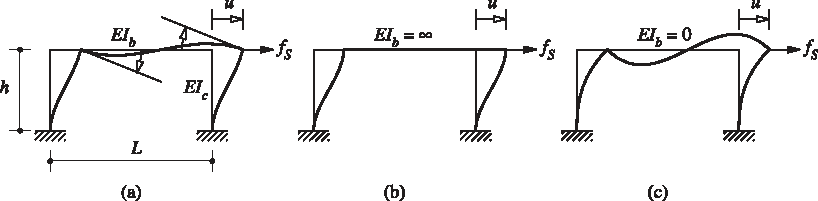
\includegraphics[width=0.9\linewidth]{frame_sdof.pdf}
	\caption{Single frame idealized as SDOF \citep{ChopraAnilK2012Dos}}
	\label{fig:frame_sdof}
\end{figure}

In the equations above, $E$ is the modulus of elasticity of steel and $I_c$ and $I_b$ are the moments of inertia of the column and beam respectively.

To determine the lateral stiffness of the frame in \cref{fig:frame_sdof} considering the real stiffness of the beam, standard procedures of static structural analysis can be used (equation below). This procedure is explained in details by \citet{ChopraAnilK2012Dos}.

\begin{gather*}
k = \frac{24 R I_c}{h^3} \frac{12 \rho + 1}{12 \rho + 4}
\end{gather*}
where $\rho$ is the beam-to-column stiffness ratio and expressed as 
\begin{gather*}
\rho = \dfrac{EI_b / L}{2 E I_c/h}
\end{gather*}

For MDOF structures the stiffness of the frame can be determined using numerical analysis. Lateral load can be applied to the top of the story of interest and then the displacement caused by the applied load will be measured. Then the accurate lateral stiffness can be calculated from the displacement caused by the lateral load. 

In the SAC examples included in this document, both extreme values of stiffness assuming $EI_b = \infty$ and $EI_b = 0$ and the actual $EI_b$ are considered. Numerical analysis employing SAP2000 \citep{sap2000} software package is used to account for the stiffness of the horizontal members for each story. \cref{tab:stiffness_3LASE} shows the story stiffness of the 3-story buildings in Seattle and Los Angeles. Actual $EI_b$ values shown in the \cref{tab:stiffness_3LASE} are based on the column and beam cross-sections provided in the \citet{FEMA335c2000}. Wherever, the column section is changing the in the mid-height of the story, the smaller cross-section is considered for the story stiffness calculations. The orientation of the column cross-sections for the moment frames are shown in \cref{fig:cols_orientation}. Note that only the stiffness of the lateral resisting elements are taken into consideration for each story stiffness and lateral stiffness of the gravity columns are ignored. Results of the story stiffness calculations for the 20-story buildings located in Seattle and Los Angeles are shown in \cref{tab:stiffness_20LASE}. The modulus of elasticity, $E$, and yield strength, $f_y$, of steel are assumed to be $29000 \ksi$ and $60 \ksi$, respectively. Values of moment of inertia for the standard steel sections given are available in \href{https://www.aisc.org/publications/steel-construction-manual-resources/}{AISC Steel Construction Manual} \citep{aiscManual}.

\begin{figure}[H]
	\begin{subfigure}[b]{0.24\linewidth}
		\centering 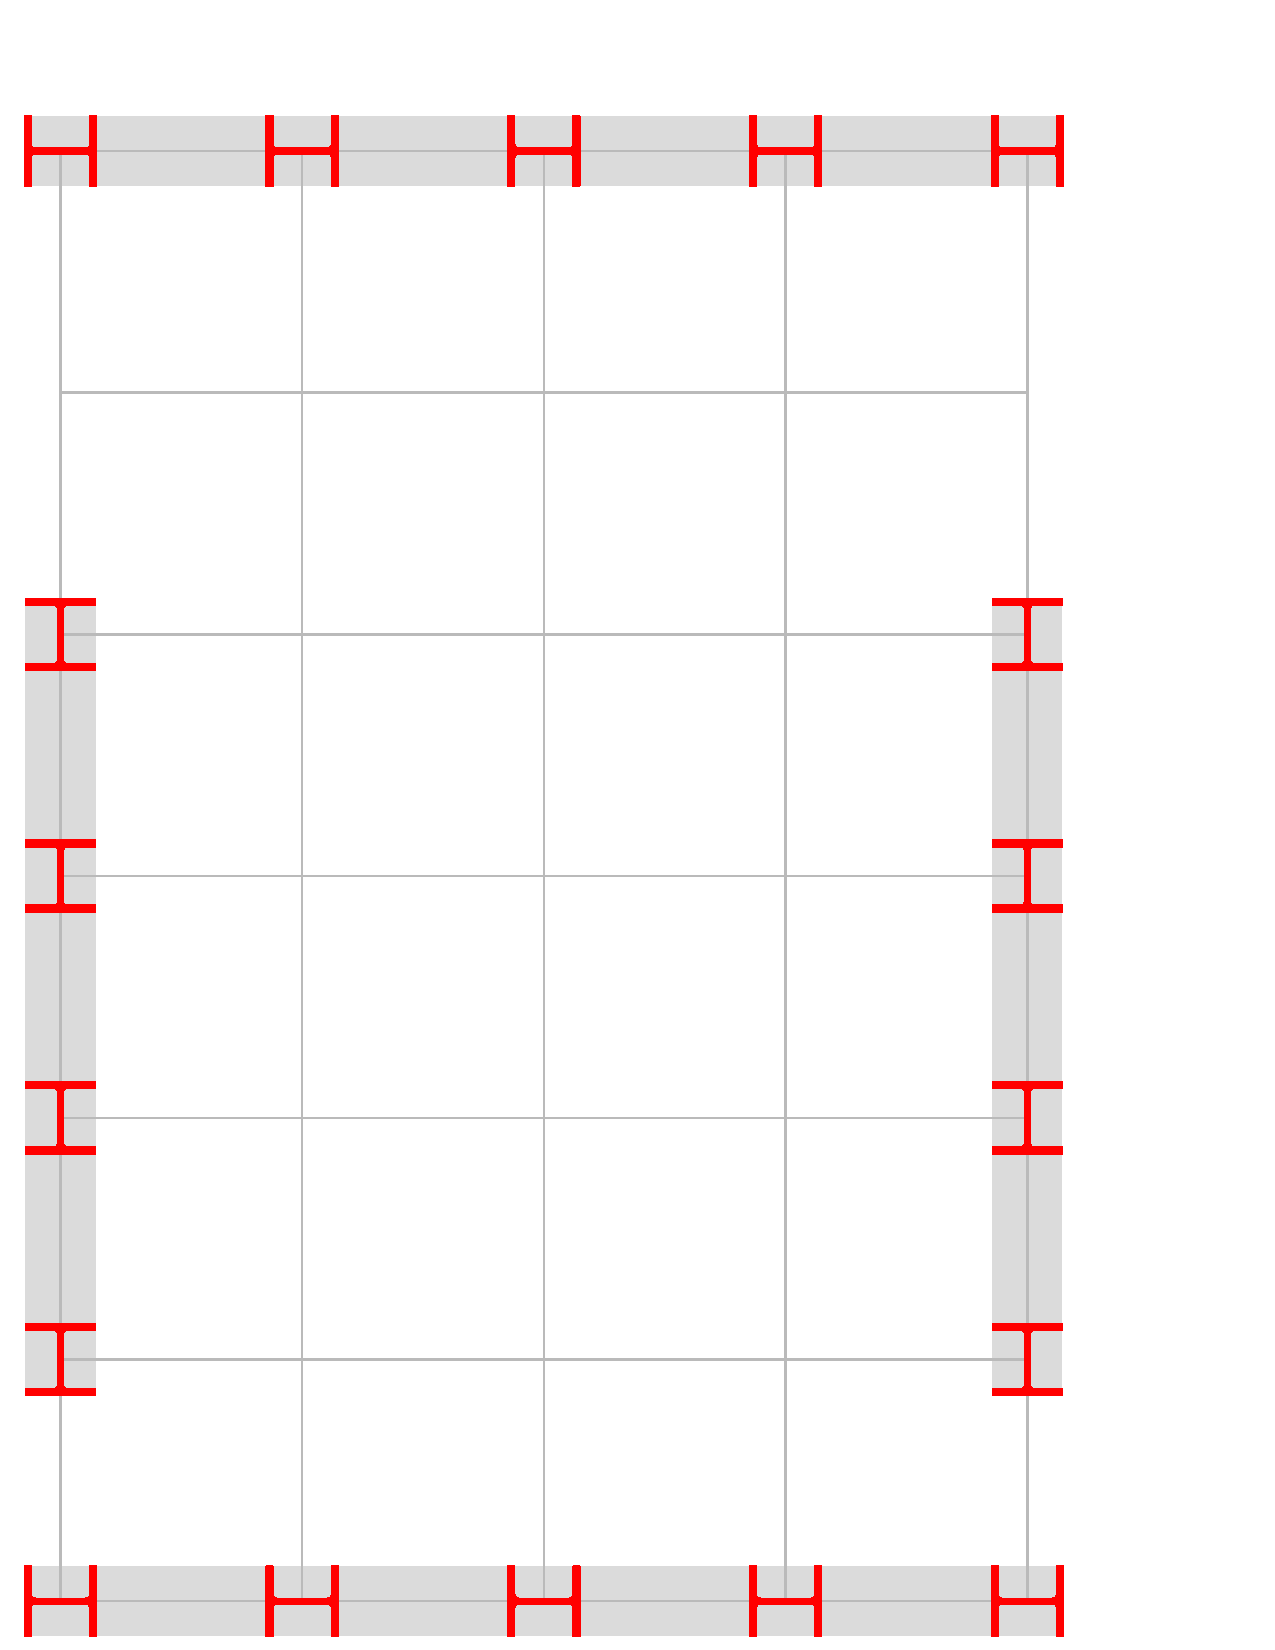
\includegraphics[page=1,trim=0mm 0mm 32mm 17mm,clip,scale=0.2]{moment_frames.pdf}
		\caption{Seattle, 3-story}
	\end{subfigure}
	\begin{subfigure}[b]{0.24\linewidth}
		\centering \includegraphics[page=2,trim=0mm 0mm 90mm 100mm,clip,scale=0.2]{moment_frames.pdf}
		\caption{Seattle, 20-story}
	\end{subfigure}
	\begin{subfigure}[b]{0.24\linewidth}
		\centering \includegraphics[page=3,trim=0mm 0mm 32mm 17mm,clip,scale=0.2]{moment_frames.pdf}
		\caption{LA, 3-story}
	\end{subfigure}
	\begin{subfigure}[b]{0.24\linewidth}
		\centering \includegraphics[page=4,trim=0mm 0mm 90mm 100mm,clip,scale=0.2]{moment_frames.pdf}
		\caption{LA, 20-story}
	\end{subfigure}
	\caption{Orientation of the columns in the moment-frames for the 3- and 20-story SAC buildings. (\textit{Note that column and beam sections for each design are available in \citet{FEMA335c2000})}.}
	\label{fig:cols_orientation}
\end{figure}


\begin{table}[H]
	\centering \caption{Story stiffness for the 3-story buildings.}
	\label{tab:stiffness_3LASE}
	\begin{tabular}{lccclccc}
	\toprule
	\multicolumn{4}{c}{Seattle}											&	\multicolumn{4}{c}{Los Angeles}	\\ \cmidrule(rl){1-4} \cmidrule(rl){5-8}
	Story	& \multicolumn{3}{c}{Stiffness, k/in.}						&	Story	& \multicolumn{3}{c}{Stiffness, k/in.}	\\ \cmidrule(rl){2-4}\cmidrule(rl){6-8}
			& $EI_b = \infty$	& actual $EI_b$		& $EI_b = 0$		&			& $EI_b = \infty$	& actual $EI_b$		& $EI_b = 0$		\\ \cmidrule(rl){1-4} \cmidrule(rl){5-8}
	1		& 5,097				& 2,918				& 1,274				& 1 \& 2	& 2,834				& 1,593				& 709				\\
	2,3		& 1,742				& 854				& 435				& 3			& 2,834				& 1,161				& 709				\\ \bottomrule
	\end{tabular}
\end{table}

\begin{table}[H]
	\centering \caption{Story stiffness for the 20-story buildings.}
	\label{tab:stiffness_20LASE}
	\begin{tabular}{lccclccc}
	\toprule
	\multicolumn{4}{c}{Seattle}						& \multicolumn{4}{c}{Los Angeles}				\\ \cmidrule(rl){1-4}\cmidrule(rl){5-8}
	Story	& \multicolumn{3}{c}{Stiffness, k/in.}						& Story		& \multicolumn{3}{c}{Stiffness, k/in.}				\\ \cmidrule(rl){2-4}\cmidrule(rl){6-8}
			& $EI_b = \infty$	& actual $EI_b$		& $EI_b = 0$		& 			& $EI_b = \infty$	& actual $EI_b$		& $EI_b = 0$\\ \cmidrule(rl){1-4}\cmidrule(rl){5-8}
	1 		& 4,434				& 2,319				& 1,108				& 1 		& 3,427				& 2,378				& 856				\\
	2 - 5	& 11,769			& 5,142				& 2,942				& 2 - 4		& 9,527				& 4,235				& 2,381				\\ 
	6 - 8	& 10,560			& 4,756				& 2,640				& 5 - 10	& 7,714				& 3,746				& 1,928				\\ 
	9 - 10	& 10,560			& 4,238				& 2,640				& 11 - 13	& 6,284				& 3,172				& 1,571				\\ 
	11 - 12	& 8,748				& 3,600				& 2,104				& 14 - 16	& 4,323				& 2,414				& 1,080				\\ 
	13 - 15	& 8,748				& 2,925				& 2,104				& 17 - 18	& 3,127				& 1,801				& 781				\\ 
	16 - 17	& 5,689				& 2,202				& 1,422				& 19		& 2,353				& 1,299				& 588				\\ 
	18 - 20	& 4,422				& 1,856				& 1,105				& 20		& 2,353				& 1,153				& 588				\\ \bottomrule
	\end{tabular}
\end{table}


%\vspace{10mm}
Thus, for this example, the input forces and building properties used in the EVW app are shown in table below. For stiffness value, actual $EI_b$ are used.

\begin{table}[H]
	\centering \caption{Input forces and building properties (3LA250).}
	\begin{tabular}{lll}
	\toprule
	\multicolumn{3}{l}{\textit{Input Forces}}					\\
	\cmidrule(rl){1-3}
	Earthquake:		& Input motion		& Northridge			\\
					& Scale factor		& 0.79					\\
	Wind:			& Exposure category	& B						\\
					& Gust wind speed	& 110.4 mph				\\
					& Seed				& 100					\\
	\midrule
	\multicolumn{3}{l}{\textit{Building Properties}}			\\
	\cmidrule(rl){1-3}
					& Number floor		& 3						\\
					& Building weight	& 6503.1 k				\\
					& shape				& Rectangular			\\
					& Height			& 468 in.				\\
					& Width				& 2160 in.				\\
					& Length			& 1440 in.				\\
					& Drag coefficient	& 1.3					\\
					& Story stiffness	& see \cref{tab:stiffness_3LASE}				\\
					& Damping ratio		& 0.02					\\
	\midrule
	\multicolumn{3}{l}{Disable PDelta effects}					\\
	\bottomrule
	\end{tabular}
\end{table}

\begin{figure}[H]
	\centering 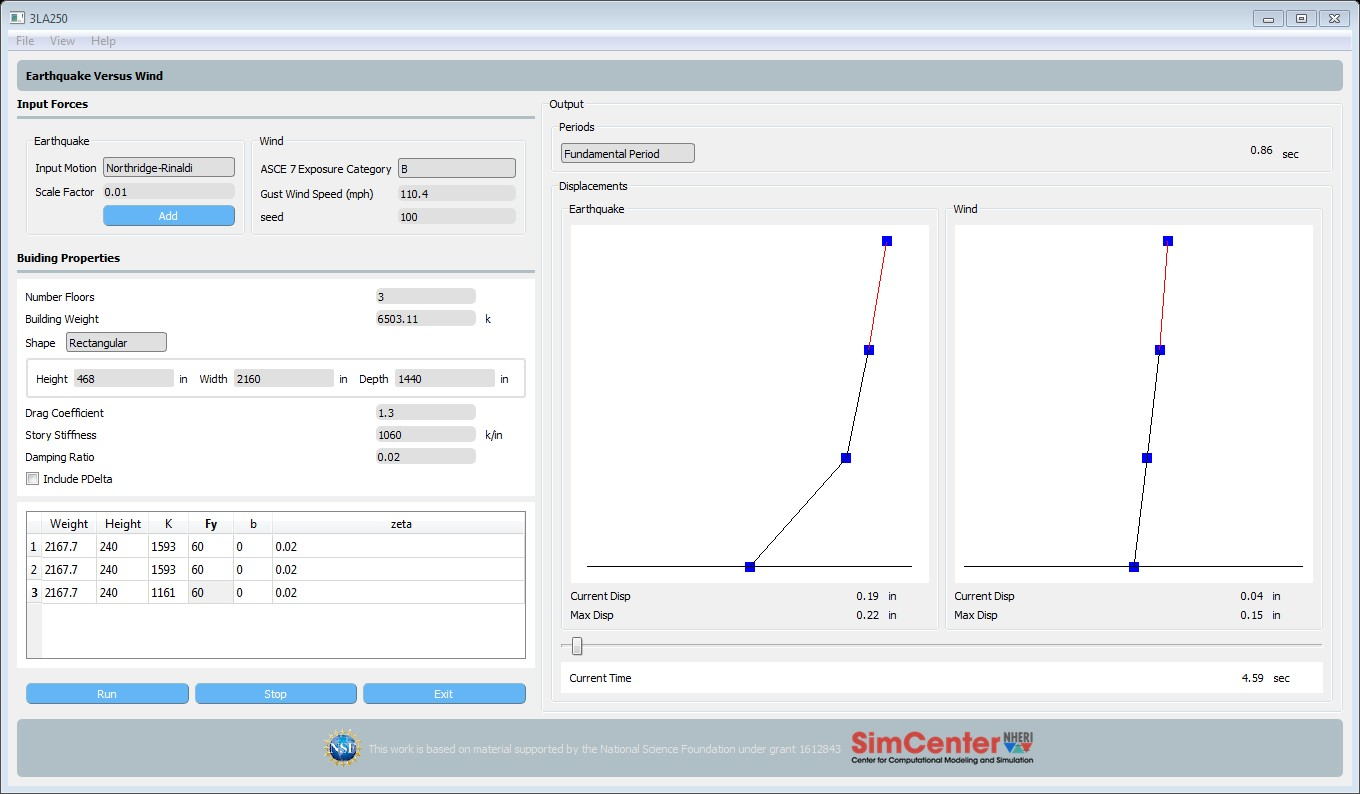
\includegraphics[width=0.9\linewidth]{3LA250_1.JPG}
	\caption{Program display after inputs entered for building 3LA250.}
\end{figure}
Following figures show some of the graphics available in the tool.
\begin{figure}[H]
	\centering 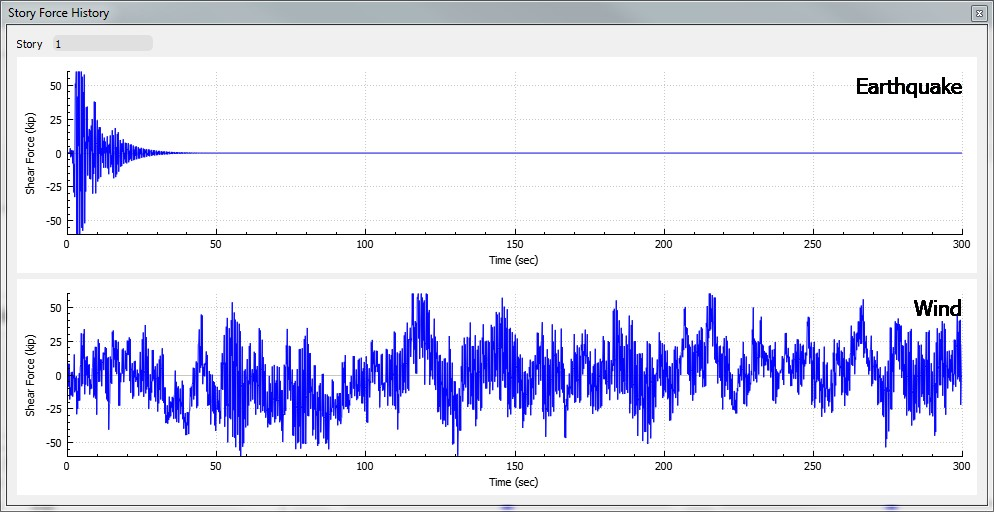
\includegraphics[scale=0.35]{3LA250_fdh.JPG}
	\caption{Floor displacement history, 3LA250, third floor.}
\end{figure}
\begin{figure}[H]
	\centering 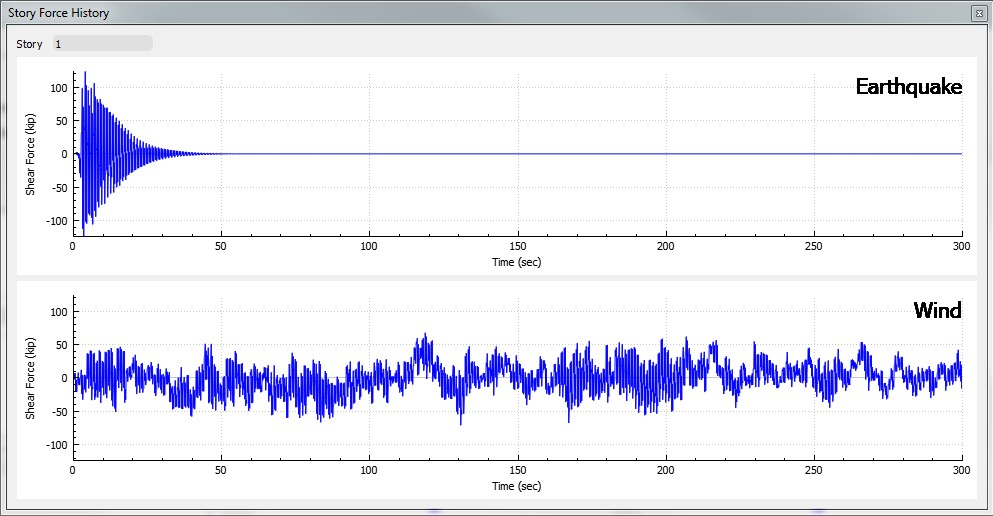
\includegraphics[scale=0.35]{3LA250_sfh.JPG}
	\caption{Story force history, 3LA250, first floor.}
\end{figure}
\begin{figure}[H]
	\centering 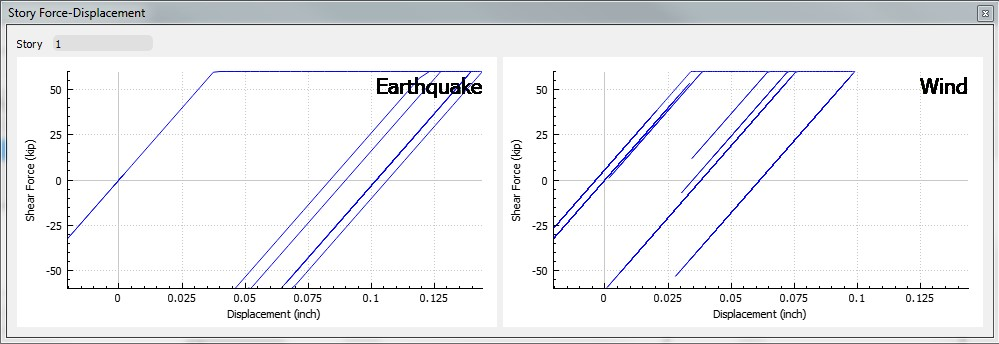
\includegraphics[scale=0.35]{3LA250_sfd.JPG}
	\caption{Story force displacement, 3LA250, first floor.}
\end{figure}
\begin{figure}[H]
	\centering 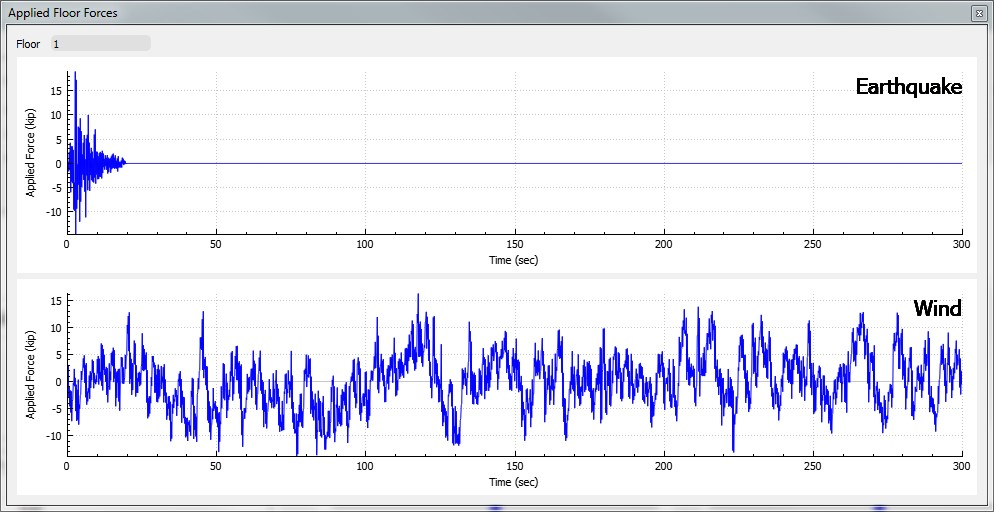
\includegraphics[scale=0.35]{3LA250_aff.JPG}
	\caption{Applied floor forces, 3LA250, first floor.}
\end{figure}




%%%%%%%%%%%%%%%%%%%%%%%%%%%%%%%%%%%%%%%%%%%%%%%%%%%%%%%%%%%%%%%%%%%%%%%%%%%%%%%%%%
%								Example 2										 %
%%%%%%%%%%%%%%%%%%%%%%%%%%%%%%%%%%%%%%%%%%%%%%%%%%%%%%%%%%%%%%%%%%%%%%%%%%%%%%%%%%

\section{The SAC 3-story Seattle Building, Hazard Level 2/50 (3SE250)}
Properties of the 3-story building located in Seattle for the hazard level of 2/50 are tabulated in \cref{tab:prop_3SE250}. These propteries are based on the location, geometry and function of the building as described in \citet{FEMA335c2000}. Floor plans, elevations and plans of moment-resisting frames for the Seattle model building are shown in \cref{fig:floor_plan_elev,fig:MRF_LASE}.

\begin{table}[H]
\centering \caption{3-story building properties, Seattle, hazard level: 2/50 (3SE250).}
\label{tab:prop_3SE250}
\begin{tabular}{llc}
\toprule
Item		& Value		& Source		\\
\midrule
Basic wind speed at reference height in exposure C	& 98 mph						& Fig. 26.5-1 ASCE 7-16		\\
Type of exposure									& $B$							& user spec					\\
$h$ Building height									& $39\ft \,(11.87\m)$			& user spec					\\
$B$ Building width									& $180\ft \,(54.79\m)$			& user spec					\\
$L$ Building depth									& $120\ft \,(36.53\m)$			& user spec					\\
$n_1$ Building natural frequency					& $2.20$ Hz						& analysis or rational approximation$^{1)}$\\
$\zeta$ Damping ratio								& $0.02$						& rational assignment$^{2)}$		\\
$C_{fx}$ Mean along-wind force coefficient			& $1.3$							& 							\\
$\beta$ Mode exponent								& $1.0$							& user spec					\\
Building density									& $1.03 \,\mathrm{slugs/ft^3}$	& bldg function				\\
%Air density											& $0.0024 \,\mathrm{slugs/ft^3}$& bldg location				\\
\bottomrule
\multicolumn{3}{l}{\footnotesize $^{1)}$ for approximate natural frequencies see section 26.11.2 and C26.11 of the ASCE 7-16. For this example, since the building}	\\
\multicolumn{3}{l}{\footnotesize \hspace{3mm} are designed and the properties of the building elements are known, the natural frequency is accurately calculated.}	\\
\multicolumn{3}{l}{\footnotesize $^{2)}$ recommended values for damping ratio can be found in Table 11.2.1, Dynamics of Structures by
Chopra, 4th ed. \citep{ChopraAnilK2012Dos}}
\end{tabular}
\end{table}

\noindent\textbf{Procedure}\\
\indent Same as the previous example, in order to use the \href{https://simcenter.designsafe-ci.org/learning-tools/evw-application/}{EVW app}, input forces and building properties need to be known. Gust-effect factor is calculated as shown in \cref{tab:gust_factor_3SE250}.

\begin{table}[H]
\centering \caption{Gust-effect factor, 3LA250.}
\label{tab:gust_factor_3SE250}
\begin{tabular}{llc}
\toprule
Item		& Value		& Source		\\
\midrule
\multicolumn{3}{l}{\textbf{FLEXIBLE BUILDING} ($all n_1$)}	\\
$\bar{z}$ Effective structure height							& $23.4 \ft$					& $0.6h$ (26.11.4 ASCE 7-16)	\\
$I_{\bar{z}}$ Turbulence intensity at eff. height				& $0.318$						& eq. 26.11.7 ASCE 7-16			\\
$L_{\bar{z}}$ Turbulence length scale at eff. height			& $285.4 \ft$					& eq. 26.11.9 ASCE 7-16			\\
$V$ Basic wind speed											& $98$ mph						& Fig. 26.5-1 ASCE 7-16			\\
$\beta$ Damping ratio											& $0.02$						& rational assignment			\\
$\bar{\alpha}$ Power law exponent of mean wind speed profile	& $0.25$						& Table 26.11-1 ASCE 7-16		\\
$\bar{b}$ Gust factor 1/F at 10 m								& $0.45$						& Table 26.11-1 ASCE 7-16		\\
$\bar{V}_{\bar{z}}$ Mean wind speed at effective height			& $59.4$						& eq. 26.11-16 ASCE 7-16		\\
$N_1$ Reduced natural frequency									& $10.58$						& eq. 26.11-14 ASCE 7-16		\\
$R_n$ Resonance response factor for n							& $0.031$						& eq. 26.11-13 ASCE 7-16		\\
$\eta_h$ Vertical decay parameter								& $6.650$						& eq. 26.11-5 ASCE 7-16			\\
$\eta_B$ Cross-wind decay parameter								& $30.691$						& eq. 26.11-5 ASCE 7-16			\\
$\eta_L$ Along-wind decay parameter								& $68.498$						& eq. 26.11-5 ASCE 7-16			\\
$R_h$ Resonant factor for $h$									& $0.139$							& eq. 26.11-15a ASCE 7-16			\\
$R_B$ Resonant factor for $B$									& $0.032$							& eq. 26.11-15a ASCE 7-16			\\
$R_L$ Resonant factor for $L$									& $0.015$							& eq. 26.11-15a ASCE 7-16			\\
$R^2$ Resonant response (squared)								& $0.004$							& eq. 26.11-12 ASCE 7-16			\\
$g_R$ Resonant peak factor										& $4.373$							& eq. 26.11-11 ASCE 7-16			\\
$G_f$ Gust-effect factor										& $0.81$							& eq. 26.11-10 ASCE 7-16			\\
\bottomrule
\end{tabular}
\end{table}

Therefore, Gust wind speed in mph is:
\begin{equation*}
G_f \times C = 0.81 \times 98 = \boxed{79.4}
\end{equation*}

Thus, input forces and building properties used in the EVW app are shown in table below:

\begin{table}[H]
	\centering \caption{Input forces and building properties (3SE250).}
	\begin{tabular}{lll}
	\toprule
	\multicolumn{3}{l}{\textit{Input Forces}}					\\
	\cmidrule(rl){1-3}
	Earthquake:		& Input motion		& Northridge			\\
					& Scale factor		& 0.22					\\
	Wind:			& Exposure category	& B						\\
					& Gust wind speed	& 79.4 mph				\\
					& Seed				& 100					\\
	\midrule
	\multicolumn{3}{l}{\textit{Building Properties}}			\\
	\cmidrule(rl){1-3}
					& Number floor		& 3						\\
					& Building weight	& 6503.1 k				\\
					& shape				& Rectangular			\\
					& Height			& 468 in.				\\
					& Width				& 2160 in.				\\
					& Length			& 1440 in.				\\
					& Drag coefficient	& 1.3					\\
					& Story stiffness	& see \cref{tab:stiffness_3LASE}			\\
					& Damping ratio		& 0.02					\\
	\midrule
	\multicolumn{3}{l}{Enable PDelta effects}					\\
	\bottomrule
	\end{tabular}
\end{table}

\begin{figure}[H]
	\centering 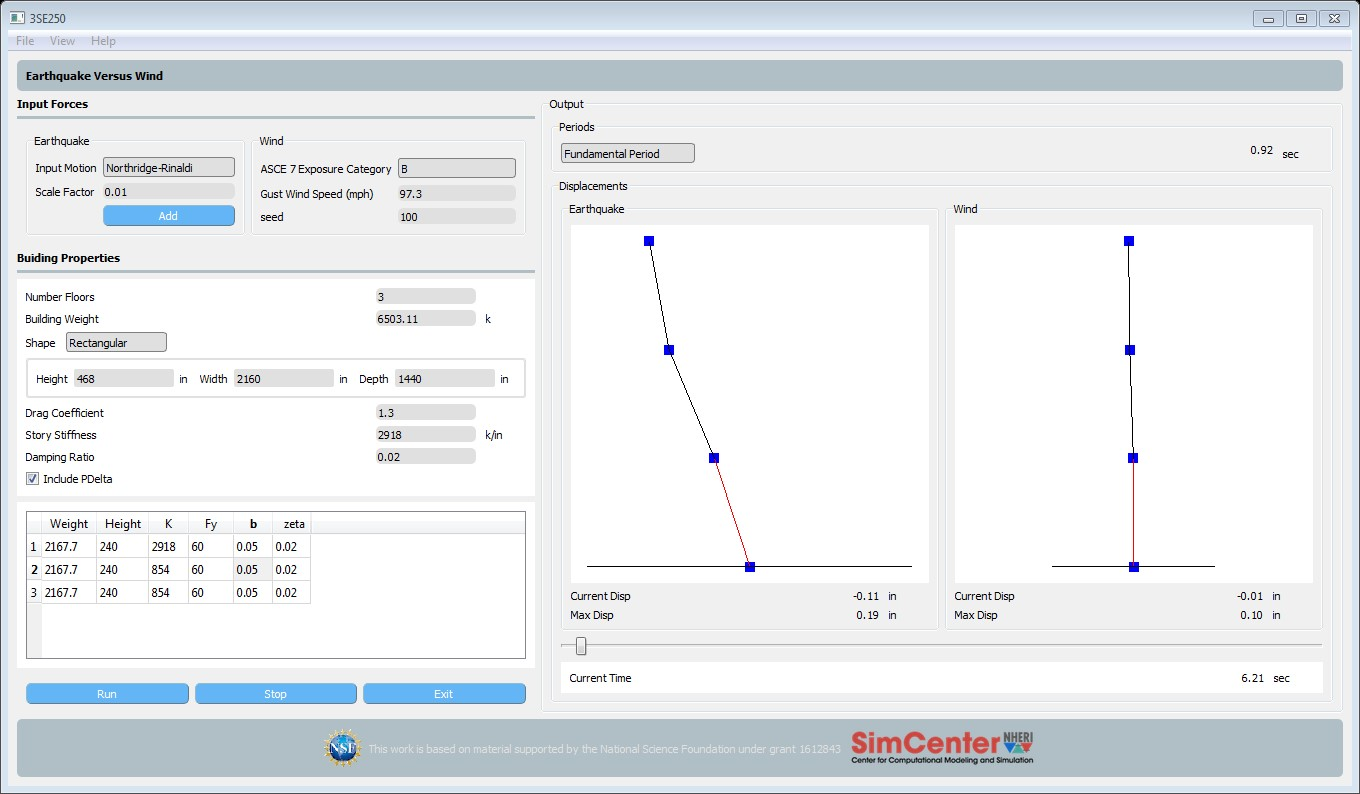
\includegraphics[width=0.9\linewidth]{3SE250_1.JPG}
	\caption{Program display after inputs entered for building 3SE250.}
\end{figure}
Following figures show some of the graphics available in the tool.
\begin{figure}[H]
	\centering 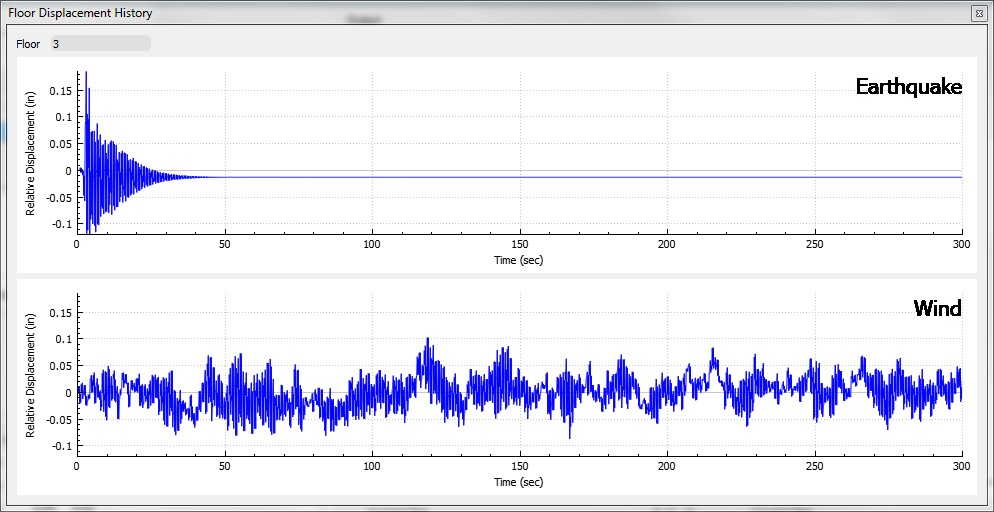
\includegraphics[scale=0.35]{3SE250_fdh.JPG}
	\caption{Floor displacement history, 3SE250, third floor.}
\end{figure}
\begin{figure}[H]
	\centering 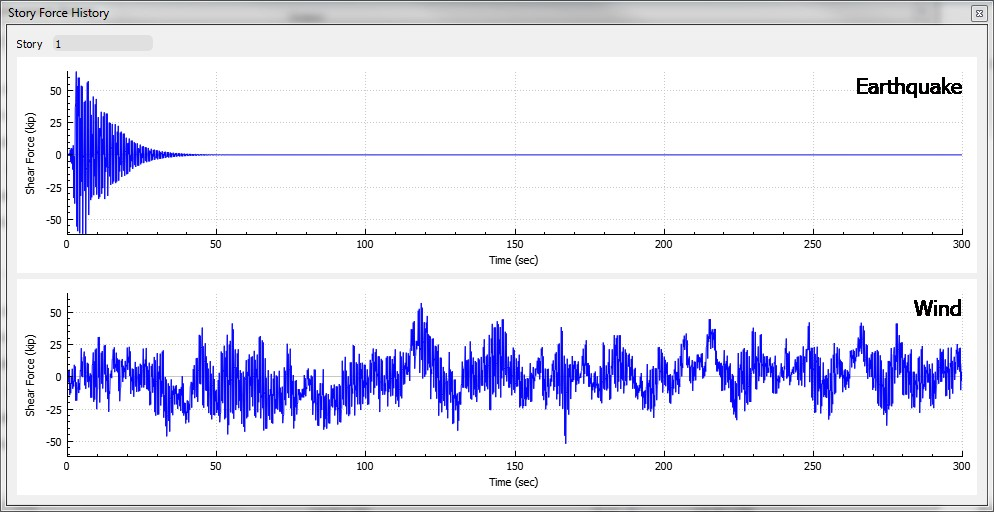
\includegraphics[scale=0.35]{3SE250_sfh.JPG}
	\caption{Story force history, 3SE250, first floor.}
\end{figure}
\begin{figure}[H]
	\centering 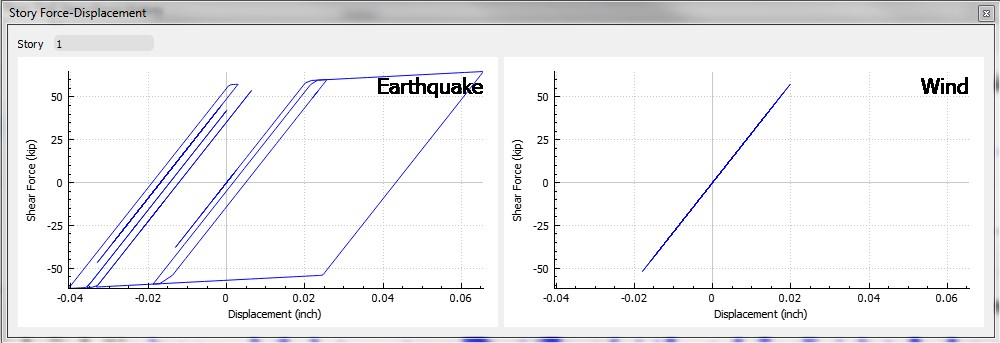
\includegraphics[scale=0.35]{3SE250_sfd.JPG}
	\caption{Story force displacement, 3SE250, first floor.}
\end{figure}
\begin{figure}[H]
	\centering 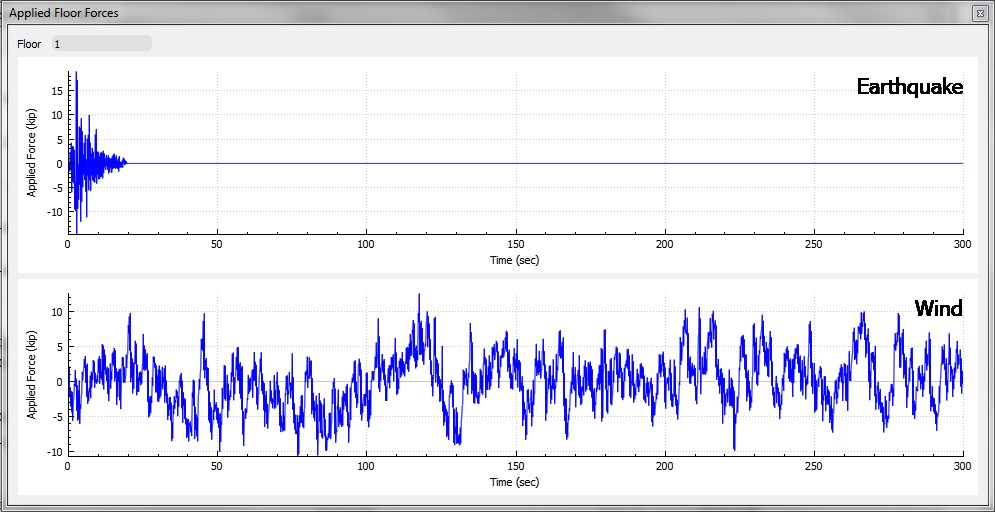
\includegraphics[scale=0.35]{3SE250_aff.JPG}
	\caption{Applied floor forces, 3SE250, first floor.}
\end{figure}




%%%%%%%%%%%%%%%%%%%%%%%%%%%%%%%%%%%%%%%%%%%%%%%%%%%%%%%%%%%%%%%%%%%%%%%%%%%%%%%%%%
%								Example 3										 %
%%%%%%%%%%%%%%%%%%%%%%%%%%%%%%%%%%%%%%%%%%%%%%%%%%%%%%%%%%%%%%%%%%%%%%%%%%%%%%%%%%

\section{The SAC 20-story Los Angeles Building, Hazard Level 2/50 (20LA250)}
Properties of the 20-story building located in Los Angeles for the hazard level of 2/50 are tabulated in \cref{tab:prop_20LA250}. Floor plans, elevations and plans of moment-resisting frames for the Seattle model building are shown in \cref{fig:floor_plan_elev,fig:MRF_LASE}.

\begin{table}[H]
\centering \caption{20-story building properties, Los Angeles, hazard level: 2/50 (20LA250).}
\label{tab:prop_20LA250}
\begin{tabular}{llc}
\toprule
Item		& Value		& Source		\\
\midrule
Basic wind speed at reference height in exposure C	& 95 mph						& Fig. 26.5-1 ASCE 7-16		\\
Type of exposure									& $B$							& user spec					\\
$h$ Building height									& $265\ft \,(80.67\m)$			& user spec					\\
$B$ Building width									& $120\ft \,(36.53\m)$			& user spec					\\
$L$ Building depth									& $100\ft \,(30.44\m)$			& user spec					\\
$n_1$ Building natural frequency					& $0.25$ Hz						& analysis or rational approximation$^{1)}$\\
$\zeta$ Damping ratio								& $0.02$						& rational assignment$^{2)}$		\\
$C_{fx}$ Mean along-wind force coefficient			& $1.3$							& 							\\
$\beta$ Mode exponent								& $1.0$							& user spec					\\
Building density									& $0.04 \,\mathrm{slugs/ft^3}$	& bldg function				\\
%Air density											& $0.0024 \,\mathrm{slugs/ft^3}$& bldg location				\\
\bottomrule
\multicolumn{3}{l}{\footnotesize $^{1)}$ for approximate natural frequencies see section 26.11.2 and C26.11 of the ASCE 7-16. For this example, since the building}	\\
\multicolumn{3}{l}{\footnotesize \hspace{3mm} are designed and the properties of the building elements are known, the natural frequency is accurately calculated.}	\\
\multicolumn{3}{l}{\footnotesize $^{2)}$ recommended values for damping ratio can be found in Table 11.2.1, Dynamics of Structures by
Chopra, 4th ed. \citep{ChopraAnilK2012Dos}}
\end{tabular}
\end{table}

\noindent\textbf{Procedure}\\
\indent Same as the previous example, in order to use the \href{https://simcenter.designsafe-ci.org/learning-tools/evw-application/}{EVW app}, input forces and building properties need to be known. Gust-effect factor is calculated as shown in \cref{tab:gust_factor_20LA250}.

\begin{table}[H]
\centering \caption{Gust-effect factor, 3LA250.}
\label{tab:gust_factor_20LA250}
\begin{tabular}{llc}
\toprule
Item		& Value		& Source		\\
\midrule
\multicolumn{3}{l}{\textbf{FLEXIBLE BUILDING} (all $n_1$)}	\\
$\bar{z}$ Effective structure height							& $159.0 \ft$					& $0.6h$ (26.11.4 ASCE 7-16)	\\
$I_{\bar{z}}$ Turbulence intensity at eff. height				& $0.231$						& eq. 26.11.7 ASCE 7-16			\\
$L_{\bar{z}}$ Turbulence length scale at eff. height			& $540.5 \ft$					& eq. 26.11.9 ASCE 7-16			\\
$V$ Basic wind speed											& $95$ mph						& Fig. 26.5-1 ASCE 7-16			\\
$\beta$ Damping ratio											& $0.02$						& rational assignment			\\
$\bar{\alpha}$ Power law exponent of mean wind speed profile	& $0.25$						& Table 26.11-1 ASCE 7-16		\\
$\bar{b}$ Gust factor 1/F at 10 m								& $0.45$						& Table 26.11-1 ASCE 7-16		\\
$\bar{V}_{\bar{z}}$ Mean wind speed at effective height			& $92.9$						& eq. 26.11-16 ASCE 7-16		\\
$N_1$ Reduced natural frequency									& $1.45$						& eq. 26.11-14 ASCE 7-16		\\
$R_n$ Resonance response factor for n							& $0.107$						& eq. 26.11-13 ASCE 7-16		\\
$\eta_h$ Vertical decay parameter								& $3.281$						& eq. 26.11-5 ASCE 7-16			\\
$\eta_B$ Cross-wind decay parameter								& $1.486$						& eq. 26.11-5 ASCE 7-16			\\
$\eta_L$ Along-wind decay parameter								& $4.145$						& eq. 26.11-5 ASCE 7-16			\\
$R_h$ Resonant factor for $h$									& $0.258$							& eq. 26.11-15a ASCE 7-16			\\
$R_B$ Resonant factor for $B$									& $0.458$							& eq. 26.11-15a ASCE 7-16			\\
$R_L$ Resonant factor for $L$									& $0.212$							& eq. 26.11-15a ASCE 7-16			\\
$R^2$ Resonant response (squared)								& $0.399$							& eq. 26.11-12 ASCE 7-16			\\
$g_R$ Resonant peak factor										& $3.845$							& eq. 26.11-11 ASCE 7-16			\\
$G_f$ Gust-effect factor										& $0.97$							& eq. 26.11-10 ASCE 7-16			\\
\bottomrule
\end{tabular}
\end{table}

Therefore, Gust wind speed in mph is:
\begin{equation*}
G_f \times C = 0.97 \times 95 = \boxed{92.2}
\end{equation*}

Thus, input forces and building properties used in the EVW app are shown in table below:

\begin{table}[H]
	\centering \caption{Input forces and building properties (20LA250).}
	\begin{tabular}{lll}
	\toprule
	\multicolumn{3}{l}{\textit{Input Forces}}					\\
	\cmidrule(rl){1-3}
	Earthquake:		& Input motion		& Northridge			\\
					& Scale factor		& 0.01					\\
	Wind:			& Exposure category	& B						\\
					& Gust wind speed	& 92.2 mph				\\
					& Seed				& 100					\\
	\midrule
	\multicolumn{3}{l}{\textit{Building Properties}}			\\
	\cmidrule(rl){1-3}
					& Number floor		& 20					\\
					& Building weight	& 24419.5 k				\\
					& shape				& Rectangular			\\
					& Height			& 3180 in.				\\
					& Width				& 1440 in.				\\
					& Length			& 1200 in.				\\
					& Drag coefficient	& 1.3					\\
					& Story stiffness	& see \cref{tab:stiffness_20LASE}			\\
					& Damping ratio		& 0.02					\\
	\midrule
	\multicolumn{3}{l}{Disable PDelta effects}					\\
	\bottomrule
	\end{tabular}
\end{table}

\begin{figure}[H]
	\centering 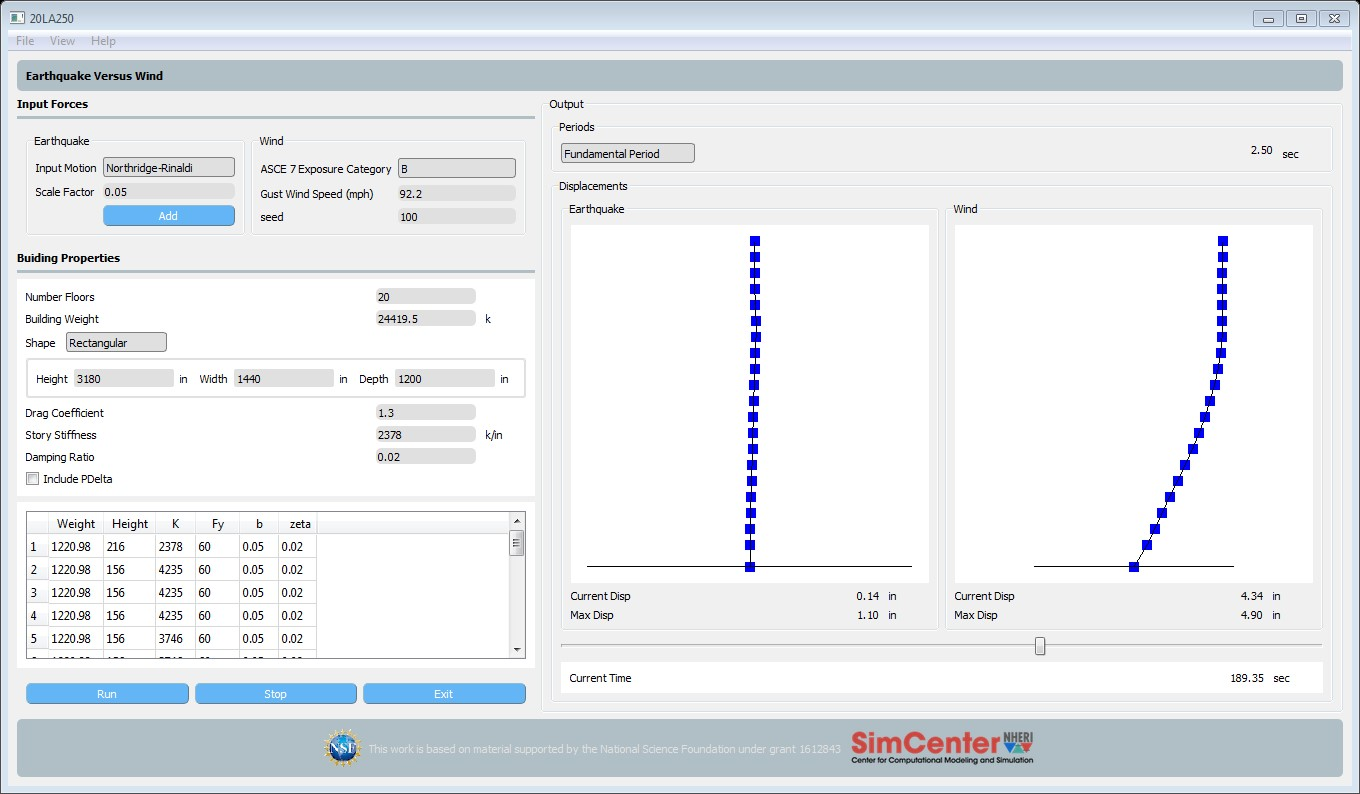
\includegraphics[width=0.9\linewidth]{20LA250_1.JPG}
	\caption{Program display after inputs entered for building 20LA250.}
\end{figure}
Following figures show some of the graphics available in the tool.
\begin{figure}[H]
	\centering 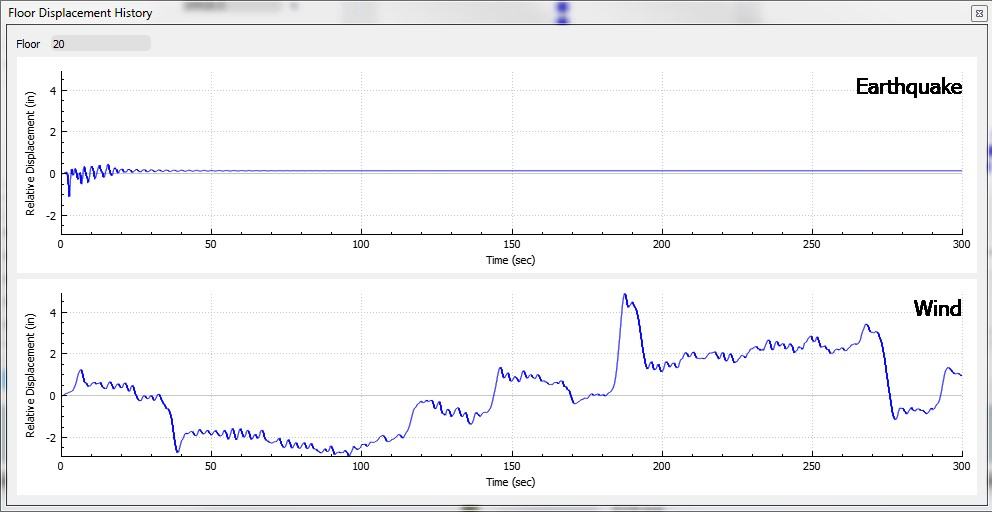
\includegraphics[scale=0.35]{20LA250_fdh.JPG}
	\caption{Floor displacement history, 20LA250, \nth{20} floor.}
\end{figure}
\begin{figure}[H]
	\centering 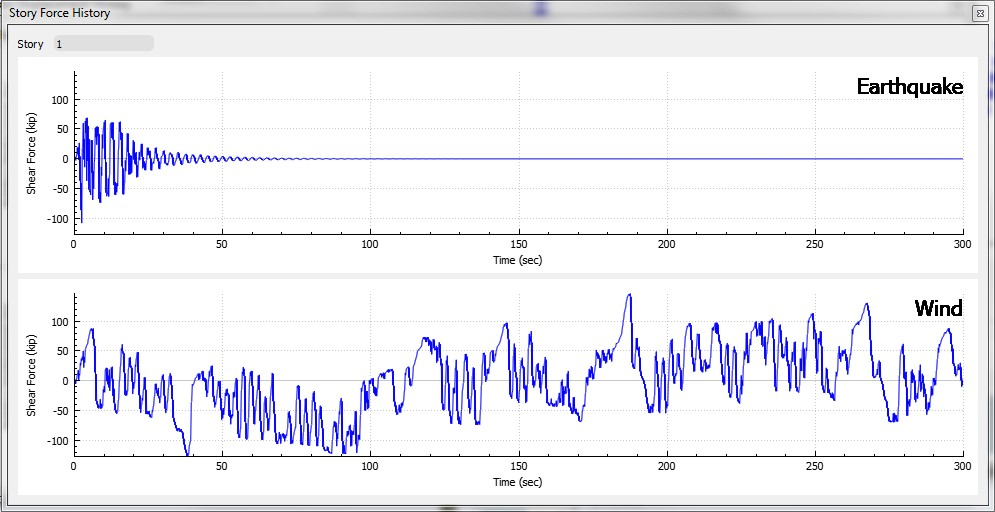
\includegraphics[scale=0.35]{20LA250_sfh.JPG}
	\caption{Story force history, 20LA250, first floor.}
\end{figure}
\begin{figure}[H]
	\centering 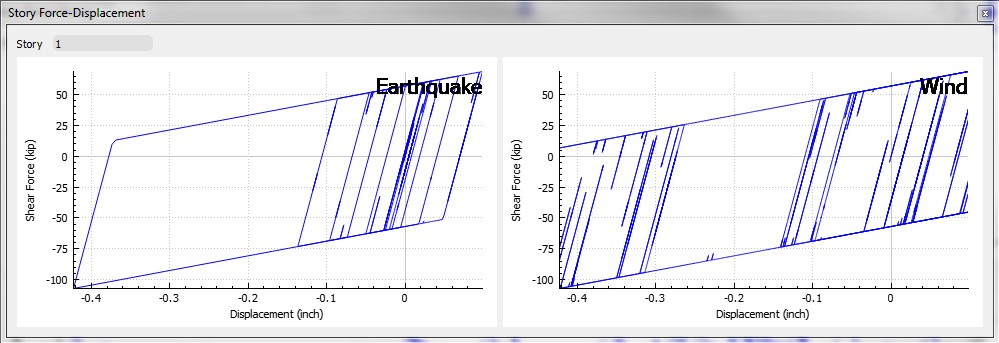
\includegraphics[scale=0.35]{20LA250_sfd.JPG}
	\caption{Story force displacement, 20LA250, first floor.}
\end{figure}
\begin{figure}[H]
	\centering 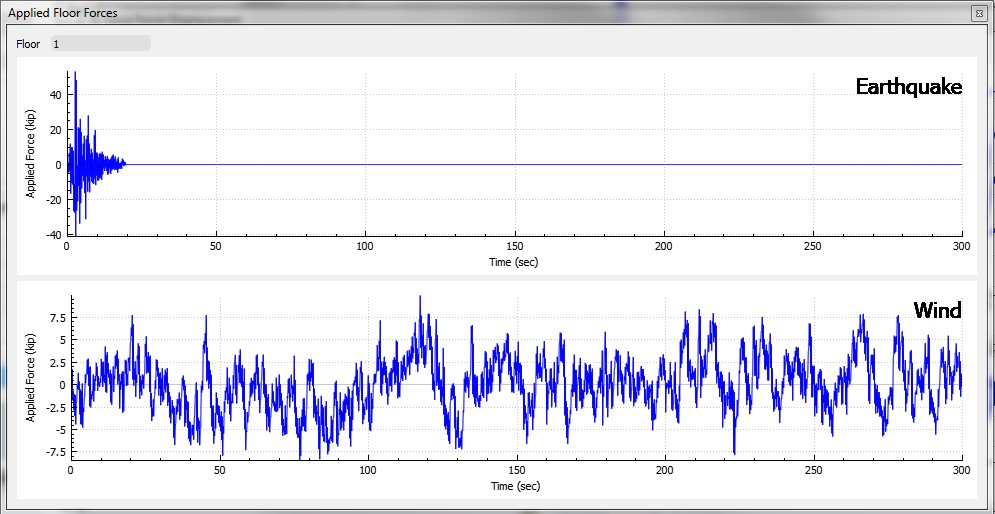
\includegraphics[scale=0.35]{20LA250_aff.JPG}
	\caption{Applied floor forces, 20LA250, first floor.}
\end{figure}




%%%%%%%%%%%%%%%%%%%%%%%%%%%%%%%%%%%%%%%%%%%%%%%%%%%%%%%%%%%%%%%%%%%%%%%%%%%%%%%%%%
%								Example 4										 %
%%%%%%%%%%%%%%%%%%%%%%%%%%%%%%%%%%%%%%%%%%%%%%%%%%%%%%%%%%%%%%%%%%%%%%%%%%%%%%%%%%

\section{The SAC 20-story Seattle Building, Hazard Level 2/50 (20SE250)}
Properties of the 20-story building located in Seattle for the hazard level of 2/50 are tabulated in \cref{tab:prop_20SE250}. See \cref{fig:floor_plan_elev,fig:MRF_LASE} for floor plans, elevations and plans of moment-resisting frames.

\begin{table}[H]
\centering \caption{20-story building properties, Seattle, hazard level: 2/50 (20SE250).}
\label{tab:prop_20SE250}
\begin{tabular}{llc}
\toprule
Item		& Value		& Source		\\
\midrule
Basic wind speed at reference height in exposure C	& 98 mph						& Fig. 26.5-1 ASCE 7-16		\\
Type of exposure									& $B$							& user spec					\\
$h$ Building height									& $265\ft \,(80.67\m)$			& user spec					\\
$B$ Building width									& $120\ft \,(36.53\m)$			& user spec					\\
$L$ Building depth									& $100\ft \,(30.44\m)$			& user spec					\\
$n_1$ Building natural frequency					& $0.26$ Hz						& analysis or rational approximation$^{1)}$\\
$\zeta$ Damping ratio								& $0.02$						& rational assignment$^{2)}$		\\
$C_{fx}$ Mean along-wind force coefficient			& $1.3$							& 							\\
$\beta$ Mode exponent								& $1.0$							& user spec					\\
Building density									& $0.04 \,\mathrm{slugs/ft^3}$	& bldg function				\\
%Air density											& $0.0024 \,\mathrm{slugs/ft^3}$& bldg location				\\
\bottomrule
\multicolumn{3}{l}{\footnotesize $^{1)}$ for approximate natural frequencies see section 26.11.2 and C26.11 of the ASCE 7-16. For this example, since the building}	\\
\multicolumn{3}{l}{\footnotesize \hspace{3mm} are designed and the properties of the building elements are known, the natural frequency is accurately calculated.}	\\
\multicolumn{3}{l}{\footnotesize $^{2)}$ recommended values for damping ratio can be found in Table 11.2.1, Dynamics of Structures by
Chopra, 4th ed. \citep{ChopraAnilK2012Dos}}
\end{tabular}
\end{table}

\noindent\textbf{Procedure}\\
\indent Same as the previous example, in order to use the \href{https://simcenter.designsafe-ci.org/learning-tools/evw-application/}{EVW app}, input forces and building properties need to be known. \cref{tab:gust_factor_20SE250} shows gust-effect factor calculations.

\begin{table}[H]
\centering \caption{Gust-effect factor, 3LA250.}
\label{tab:gust_factor_20SE250}
\begin{tabular}{llc}
\toprule
Item		& Value		& Source		\\
\midrule
\multicolumn{3}{l}{\textbf{FLEXIBLE BUILDING} (all $n_1$)}	\\
$\bar{z}$ Effective structure height							& $159.0 \ft$					& $0.6h$ (26.11.4 ASCE 7-16)	\\
$I_{\bar{z}}$ Turbulence intensity at eff. height				& $0.231$						& eq. 26.11.7 ASCE 7-16			\\
$L_{\bar{z}}$ Turbulence length scale at eff. height			& $540.5 \ft$					& eq. 26.11.9 ASCE 7-16			\\
$V$ Basic wind speed											& $98$ mph						& Fig. 26.5-1 ASCE 7-16			\\
$\beta$ Damping ratio											& $0.02$						& rational assignment			\\
$\bar{\alpha}$ Power law exponent of mean wind speed profile	& $0.25$						& Table 26.11-1 ASCE 7-16		\\
$\bar{b}$ Gust factor 1/F at 10 m								& $0.45$						& Table 26.11-1 ASCE 7-16		\\
$\bar{V}_{\bar{z}}$ Mean wind speed at effective height			& $95.8$						& eq. 26.11-16 ASCE 7-16		\\
$N_1$ Reduced natural frequency									& $1.47$						& eq. 26.11-14 ASCE 7-16		\\
$R_n$ Resonance response factor for n							& $0.107$						& eq. 26.11-13 ASCE 7-16		\\
$\eta_h$ Vertical decay parameter								& $3.307$						& eq. 26.11-5 ASCE 7-16			\\
$\eta_B$ Cross-wind decay parameter								& $1.498$						& eq. 26.11-5 ASCE 7-16			\\
$\eta_L$ Along-wind decay parameter								& $4.178$						& eq. 26.11-5 ASCE 7-16			\\
$R_h$ Resonant factor for $h$									& $0.257$							& eq. 26.11-15a ASCE 7-16			\\
$R_B$ Resonant factor for $B$									& $0.456$							& eq. 26.11-15a ASCE 7-16			\\
$R_L$ Resonant factor for $L$									& $0.211$							& eq. 26.11-15a ASCE 7-16			\\
$R^2$ Resonant response (squared)								& $0.393$							& eq. 26.11-12 ASCE 7-16			\\
$g_R$ Resonant peak factor										& $3.855$							& eq. 26.11-11 ASCE 7-16			\\
$G_f$ Gust-effect factor										& $0.97$							& eq. 26.11-10 ASCE 7-16			\\
\bottomrule
\end{tabular}
\end{table}

Therefore, Gust wind speed in mph is:
\begin{equation*}
G_f \times C = 0.97 \times 98 = \boxed{95.0}
\end{equation*}

Thus, input forces and building properties used in the EVW app are shown in table below:

\begin{table}[H]
	\centering \caption{Input forces and building properties (20SE250).}
	\begin{tabular}{lll}
	\toprule
	\multicolumn{3}{l}{\textit{Input Forces}}					\\
	\cmidrule(rl){1-3}
	Earthquake:		& Input motion		& Northridge			\\
					& Scale factor		& 0.01					\\
	Wind:			& Exposure category	& B						\\
					& Gust wind speed	& 95.0 mph				\\
					& Seed				& 100					\\
	\midrule
	\multicolumn{3}{l}{\textit{Building Properties}}			\\
	\cmidrule(rl){1-3}
					& Number floor		& 20					\\
					& Building weight	& 24419.5 k				\\
					& shape				& Rectangular			\\
					& Height			& 3180 in.				\\
					& Width				& 1440 in.				\\
					& Length			& 1200 in.				\\
					& Drag coefficient	& 1.3					\\
					& Story stiffness	& see \cref{tab:stiffness_20LASE}			\\
					& Damping ratio		& 0.02					\\
	\midrule
	\multicolumn{3}{l}{Disable PDelta effects}					\\
	\bottomrule
	\end{tabular}
\end{table}

\begin{figure}[H]
	\centering 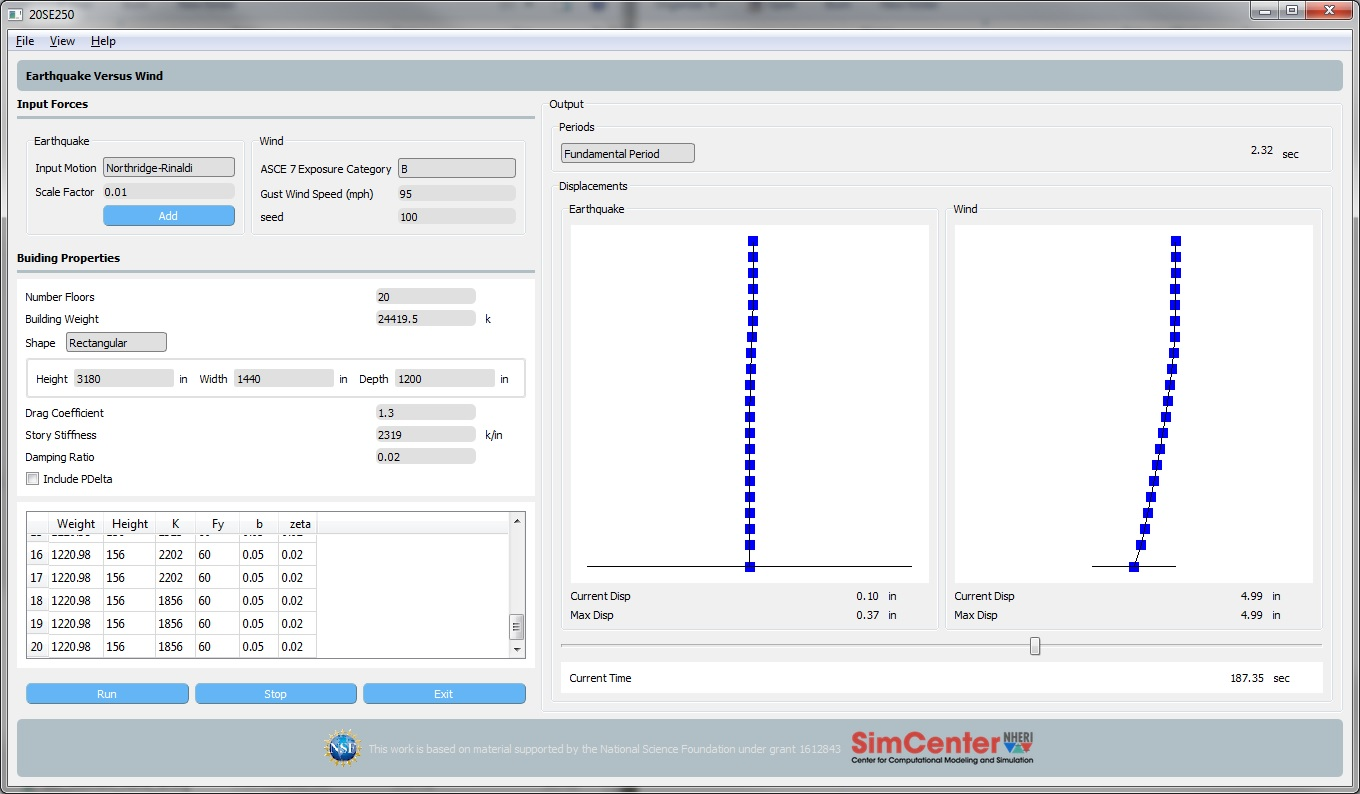
\includegraphics[width=0.9\linewidth]{20SE250_1.JPG}
	\caption{Program display after inputs entered for building 20SE250.}
\end{figure}
Following figures show some of the graphics available in the tool.
\begin{figure}[H]
	\centering 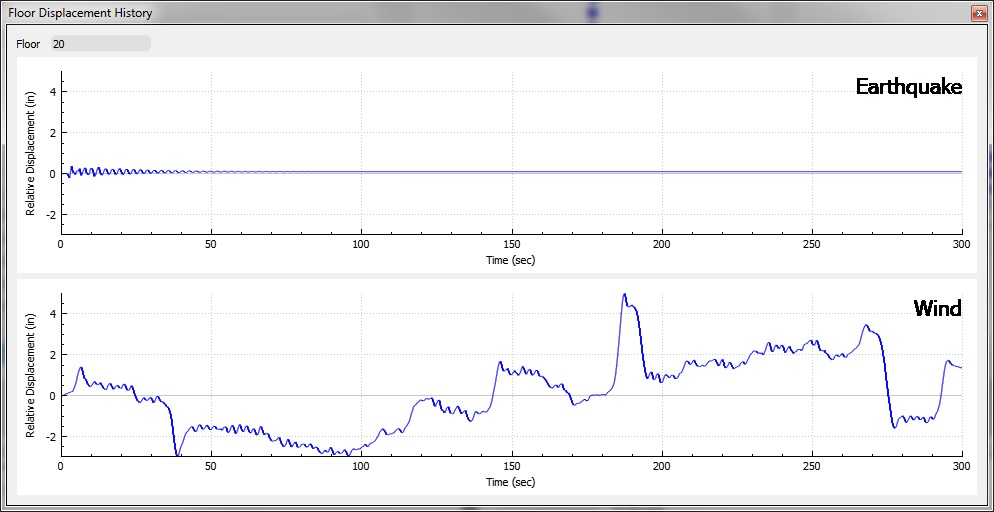
\includegraphics[scale=0.35]{20SE250_fdh.JPG}
	\caption{Floor displacement history, 20SE250, \nth{20} floor.}
\end{figure}
\begin{figure}[H]
	\centering 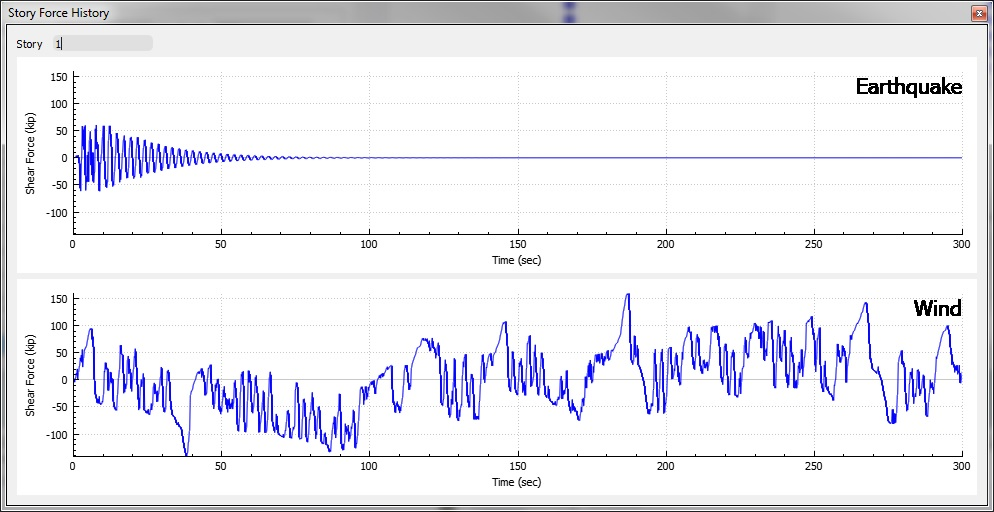
\includegraphics[scale=0.35]{20SE250_sfh.JPG}
	\caption{Story force history, 20SE250, first floor.}
\end{figure}
\begin{figure}[H]
	\centering 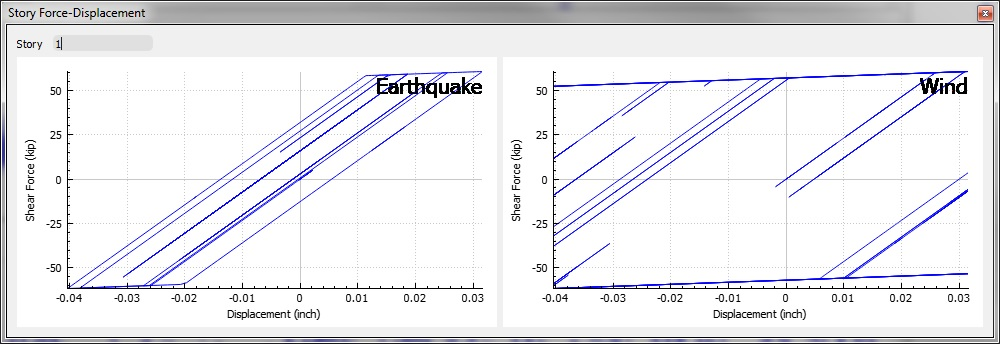
\includegraphics[scale=0.35]{20SE250_sfd.JPG}
	\caption{Story force displacement, 20SE250, first floor.}
\end{figure}
\begin{figure}[H]
	\centering 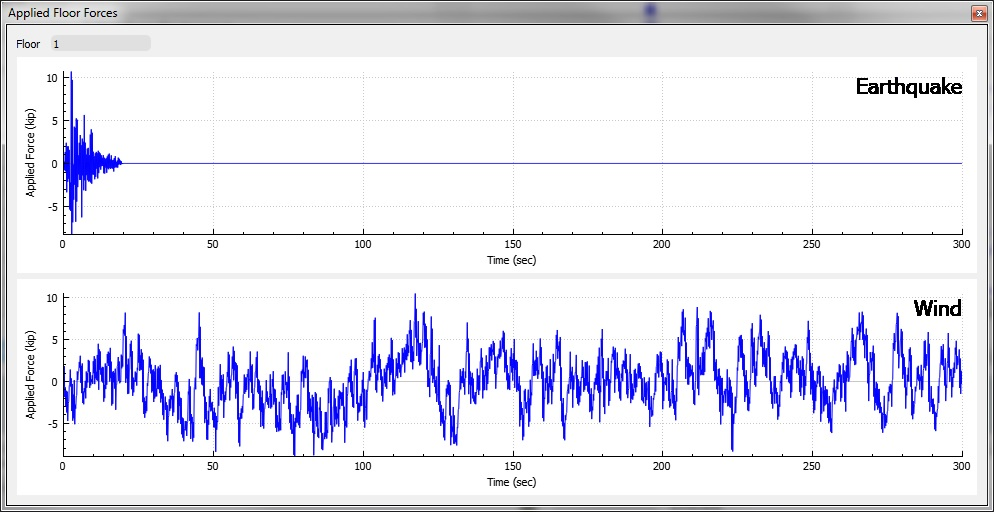
\includegraphics[scale=0.35]{20SE250_aff.JPG}
	\caption{Applied floor forces, 20SE250, \nth{20} floor.}
\end{figure}




%%%%%%%%%%%%%%%%%%%%%%%%%%%%%%%%%%%%%%%%%%%%%%%%%%%%%%%%%%%%%%%%%%%%%%%%%%%%%%%%%%
%					Example 5 Walled Building									 %
%%%%%%%%%%%%%%%%%%%%%%%%%%%%%%%%%%%%%%%%%%%%%%%%%%%%%%%%%%%%%%%%%%%%%%%%%%%%%%%%%%

\section{Walled Building}
In this example, an 8-story walled building is taken into consideration where only the walls contribute to the lateral resistance. Therefore, for stiffness consideration, only walls will be considered. Floor plan and elevation of the building and locations of walls are shown in \cref{fig:8_floor_plan}. The building is located in Los Angeles. This example is adopted from  the final report for the Applied Technology Council’s project (ATC123 project); (Report to project technical committee and project review) \citep{FEMAp2012}.

To find the stiffness of this building, as explained earlier, point loads were applied at top of the first story and then the stiffness was calculated based on the displacements caused by the point loads.

\begin{figure}[H]
	\begin{subfigure}[b]{0.7\linewidth}
		\centering \includegraphics[trim=40mm 20mm 50mm 20mm,clip,scale=0.35]{Reinforcement_Details_8story.pdf}
		\caption{Plan}	
	\end{subfigure}
	\begin{subfigure}[b]{0.25\linewidth}
		\centering 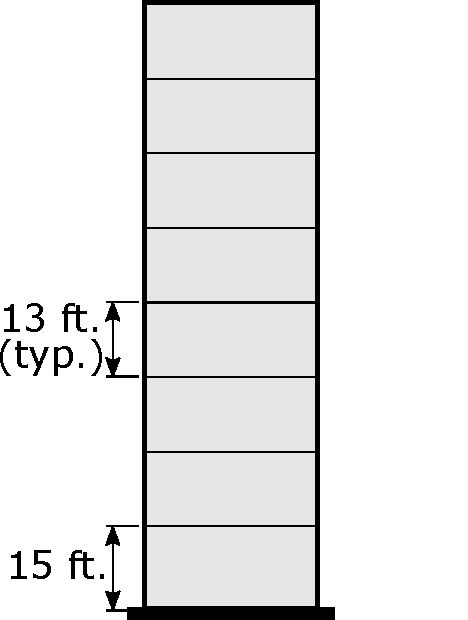
\includegraphics[scale=0.5]{bldg_elevations.pdf}
		\caption{Elevation}
	\end{subfigure}
	\caption{Floor plan and elevation of the 8-story walled building.}
	\label{fig:8_floor_plan}
\end{figure}

Properties of the 8-story walled building is shown in table below.
\begin{table}[H]
\centering \caption{8-story walled building properties.}
\begin{tabular}{llc}
\toprule
Item		& Value		& Source		\\
\midrule
Basic wind speed at reference height in exposure C	& 95 mph						& Fig. 26.5-1 ASCE 7-16		\\
Type of exposure									& $B$							& user spec					\\
$h$ Building height									& $106\ft \,(32.27\m)$			& user spec					\\
$B$ Building width									& $120\ft \,(36.53\m)$			& user spec					\\
$L$ Building depth									& $120\ft \,(36.53\m)$			& user spec					\\
$n_1$ Building natural frequency					& $0.88$ Hz						& analysis or rational approximation$^{1)}$\\
$\zeta$ Damping ratio								& $0.02$						& rational assignment$^{2)}$		\\
$C_{fx}$ Mean along-wind force coefficient			& $1.3$							& 							\\
$\beta$ Mode exponent								& $1.0$							& user spec					\\
Building density									& $0.433 \,\mathrm{slugs/ft^3}$	& bldg function				\\
%Air density											& $0.0024 \,\mathrm{slugs/ft^3}$& bldg location				\\
\bottomrule
\multicolumn{3}{l}{\footnotesize $^{1)}$ for approximate natural frequencies see section 26.11.2 and C26.11 of the ASCE 7-16. For this example, since the building}	\\
\multicolumn{3}{l}{\footnotesize \hspace{3mm} are designed and the properties of the building elements are known, the natural frequency is accurately calculated.}	\\
\multicolumn{3}{l}{\footnotesize $^{2)}$ recommended values for damping ratio can be found in Table 11.2.1, Dynamics of Structures by
Chopra, 4th ed. \citep{ChopraAnilK2012Dos}}
\end{tabular}
\end{table}

\noindent\textbf{Procedure}\\
\indent Same as the previous example, in order to use the \href{https://simcenter.designsafe-ci.org/learning-tools/evw-application/}{EVW app}, input forces and building properties need to be known. \cref{tab:gust_factor_8_story_bldg} shows gust-effect factor calculations.

\begin{table}[H]
\centering \caption{Gust-effect factor, 3LA250.}
\label{tab:gust_factor_8_story_bldg}
\begin{tabular}{llc}
\toprule
Item		& Value		& Source		\\
\midrule
\multicolumn{3}{l}{\textbf{FLEXIBLE BUILDING} (all $n_1$)}	\\
$\bar{z}$ Effective structure height							& $63.6 \ft$					& $0.6h$ (26.11.4 ASCE 7-16)	\\
$I_{\bar{z}}$ Turbulence intensity at eff. height				& $0.267$						& eq. 26.11.7 ASCE 7-16			\\
$L_{\bar{z}}$ Turbulence length scale at eff. height			& $398.2 \ft$					& eq. 26.11.9 ASCE 7-16			\\
$V$ Basic wind speed											& $95$ mph						& Fig. 26.5-1 ASCE 7-16			\\
$\beta$ Damping ratio											& $0.02$						& rational assignment			\\
$\bar{\alpha}$ Power law exponent of mean wind speed profile	& $0.25$						& Table 26.11-1 ASCE 7-16		\\
$\bar{b}$ Gust factor 1/F at 10 m								& $0.45$						& Table 26.11-1 ASCE 7-16		\\
$\bar{V}_{\bar{z}}$ Mean wind speed at effective height			& $73.9$						& eq. 26.11-16 ASCE 7-16		\\
$N_1$ Reduced natural frequency									& $4.74$						& eq. 26.11-14 ASCE 7-16		\\
$R_n$ Resonance response factor for n							& $0.052$						& eq. 26.11-13 ASCE 7-16		\\
$\eta_h$ Vertical decay parameter								& $5.808$						& eq. 26.11-5 ASCE 7-16			\\
$\eta_B$ Cross-wind decay parameter								& $6.575$						& eq. 26.11-5 ASCE 7-16			\\
$\eta_L$ Along-wind decay parameter								& $22.013$						& eq. 26.11-5 ASCE 7-16			\\
$R_h$ Resonant factor for $h$									& $0.157$							& eq. 26.11-15a ASCE 7-16			\\
$R_B$ Resonant factor for $B$									& $0.141$							& eq. 26.11-15a ASCE 7-16			\\
$R_L$ Resonant factor for $L$									& $0.044$							& eq. 26.11-15a ASCE 7-16			\\
$R^2$ Resonant response (squared)								& $0.032$							& eq. 26.11-12 ASCE 7-16			\\
$g_R$ Resonant peak factor										& $4.159$							& eq. 26.11-11 ASCE 7-16			\\
$G_f$ Gust-effect factor										& $0.85$							& eq. 26.11-10 ASCE 7-16			\\
\bottomrule
\end{tabular}
\end{table}

Therefore, Gust wind speed in mph is:
\begin{equation*}
G_f \times C = 0.85 \times 95 = \boxed{80.75}
\end{equation*}

Thus, input forces and building properties used in the EVW app are shown in table below:

\begin{table}[H]
	\centering \caption{Input forces and building properties (20SE250).}
	\begin{tabular}{lll}
	\toprule
	\multicolumn{3}{l}{\textit{Input Forces}}					\\
	\cmidrule(rl){1-3}
	Earthquake:		& Input motion		& Northridge			\\
					& Scale factor		& 0.01					\\
	Wind:			& Exposure category	& B						\\
					& Gust wind speed	& 95.0 mph				\\
					& Seed				& 100					\\
	\midrule
	\multicolumn{3}{l}{\textit{Building Properties}}			\\
	\cmidrule(rl){1-3}
					& Number floor		& 8						\\
					& Building weight	& 21276.0 k				\\
					& shape				& Rectangular			\\
					& Height			& 1272 in.				\\
					& Width				& 1440 in.				\\
					& Drag coefficient	& 1.3					\\
					& Story stiffness	& 6200.0 k/in.			\\
					& Damping ratio		& 0.02					\\
	\midrule
	\multicolumn{3}{l}{Enable PDelta effects}					\\
	\bottomrule
	\end{tabular}
\end{table}

\begin{figure}[H]
	\centering 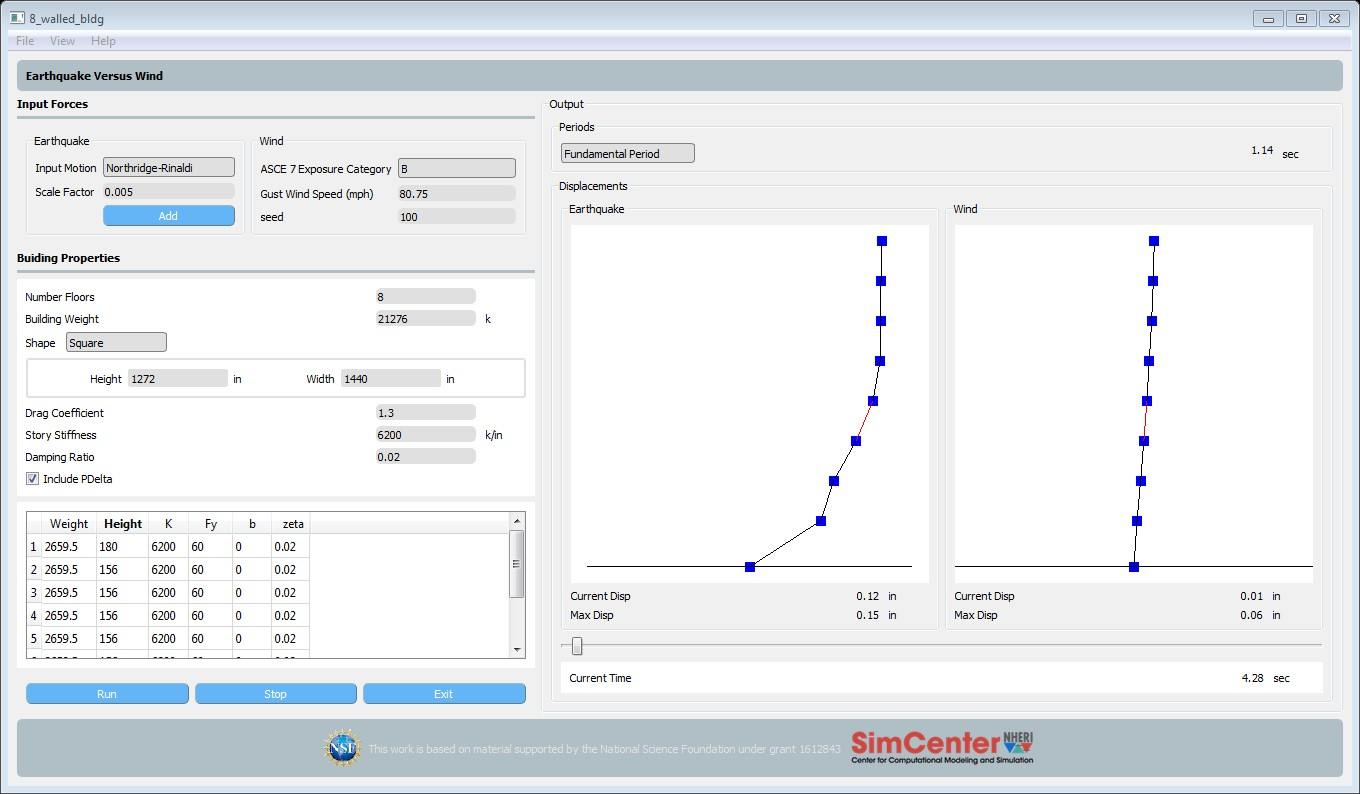
\includegraphics[width=0.9\linewidth]{8_walled_bldg_1.JPG}
	\caption{Program display after inputs entered for 8-story walled building.}
\end{figure}
Following figures show some of the graphics available in the tool.
\begin{figure}[H]
	\centering 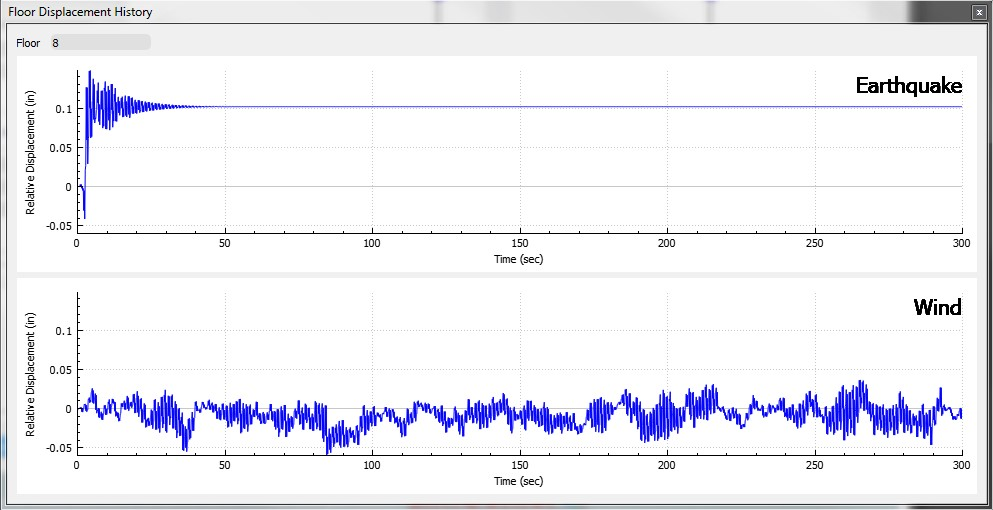
\includegraphics[scale=0.35]{8_walled_bldg_fdh.JPG}
	\caption{Floor displacement history, 8-story walled biuilding, \nth{8} floor.}
\end{figure}
\begin{figure}[H]
	\centering 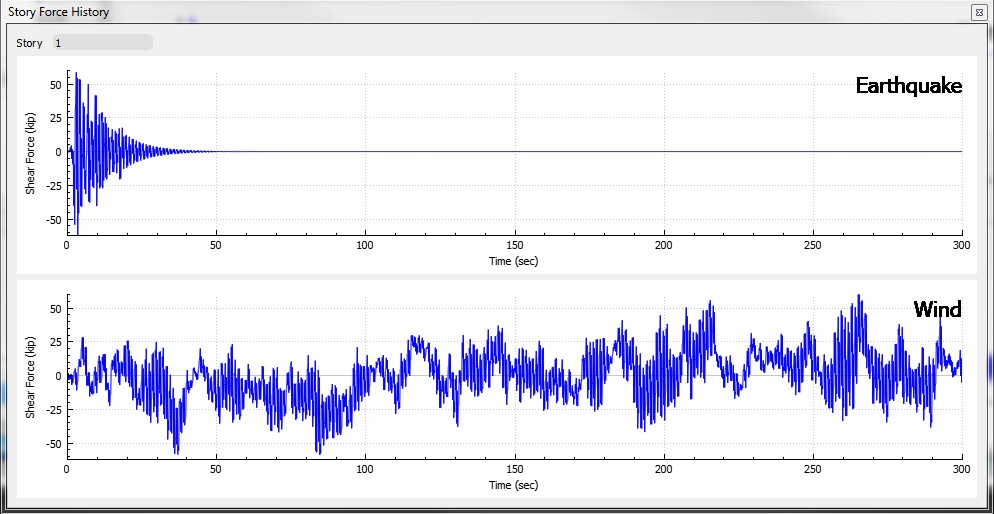
\includegraphics[scale=0.35]{8_walled_bldg_sfh.JPG}
	\caption{Story force history, 8-story walled biuilding, first floor.}
\end{figure}
\begin{figure}[H]
	\centering 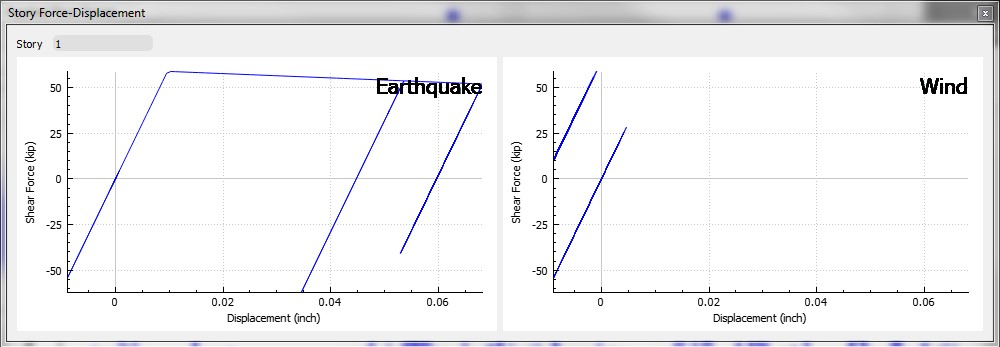
\includegraphics[scale=0.35]{8_walled_bldg_sfd.JPG}
	\caption{Story force displacement, 8-story walled biuilding, first floor.}
\end{figure}
\begin{figure}[H]
	\centering 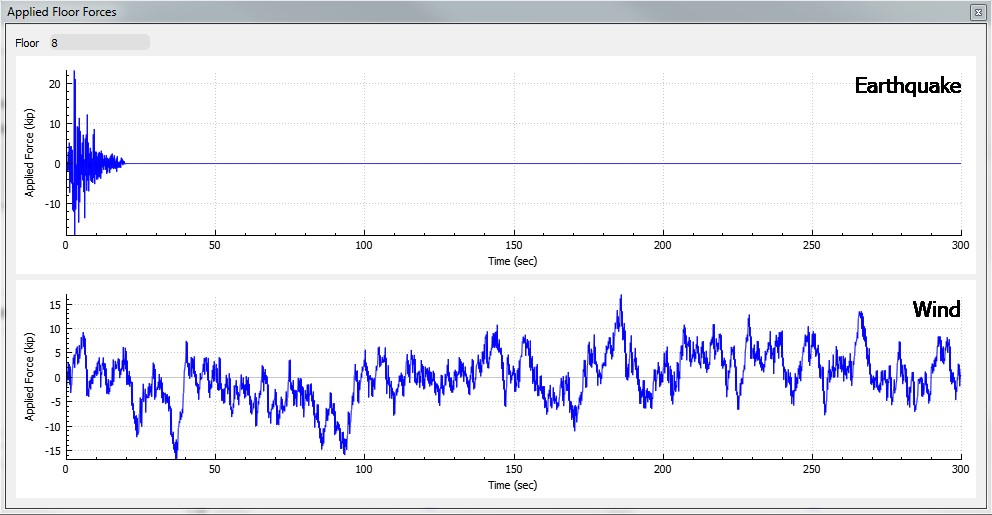
\includegraphics[scale=0.35]{8_walled_bldg_aff.JPG}
	\caption{Applied floor forces, 8-story walled biuilding, \nth{8} floor.}
\end{figure}



%%%%%%%%%%%%%%%%%%%%%%%%%%%%%%%%%%%%%%%%%%%%%%%%%%%%%%%%%%%%%%%%%%%%%%%%%%%%%%%%%%
%								references									 %
%%%%%%%%%%%%%%%%%%%%%%%%%%%%%%%%%%%%%%%%%%%%%%%%%%%%%%%%%%%%%%%%%%%%%%%%%%%%%%%%%%

\newpage
%\section{REFERENCES}
%\bibliographystyle{ieeetr}
\bibliographystyle{plainnat}
\bibliography{references}
\addcontentsline{toc}{section}{References}

\end{document}